\documentclass[../thesis_seyed.tex]{subfiles}
% \graphicspath{{\subfix{../img/}}}
\begin{document}
\chapter{OLDER ADULTS USE FEWER MUSCLES TO OVERCOME PERTURBATIONS DURING A SEATED LOCOMOTOR TASK}
\section{Introduction}

Muscle co-contraction, i.e., the concurrent activity of the agonist and antagonist muscles, is a common strategy when responding to motor perturbations and during increased uncertainty; this co-contraction usually decreases with the progression of adaptation and reduction of motor errors in response to the perturbations \cite{Thoroughman1999-pz,Huang2012-dr}. Young adults seem to use co-contraction more strategically to adapt more rapidly to perturbations and improve their accuracy in upper limb reaching tasks \cite{Gribble2003-tj,Heald2018-ko}. Young adults initially increase their muscular activity in response to postural balance challenges and split-belt walking \cite{Finley2013-lu,Kim2018-jj}. This muscular activity gradually decreases after adapting to the perturbations and reducing motor errors. However, young adults may not reduce their co-contraction as they adapt to standing or walking perturbations \cite{Kim2018-jj,Acuna2019-lo}.

Older adults often use more global co-contraction compared to young adults, presumably to resist perturbations \cite{Huang2014-nh,Iwamoto2017-ji,Thompson2018-ku}. During perturbed goal-directed reaching tasks, older adults did not reduce their motor errors or co-contraction as much as young adults \cite{Huang2014-nh,Wittenberg2020-bz}. During postural and locomotor perturbations, older adults also used more co-contraction, indicating an increased effort to adapt to the perturbations \cite{Iwamoto2017-ji,Acuna2019-lo}. An undesirable consequence of the increased co-contraction during postural tasks is that it may reduce balance performance, particularly in older adults \cite{Nagai2017-ul}. The increased co-contraction during balance tasks and walking in older adults seems to be an age-specific strategy, which is not due to a lack of sensory acuity and might be insufficient to respond to losses of balance \cite{Tang1998-jp,Craig2016-wh,Nagai2017-ul,Thompson2018-ku,Le_Mouel2019-wf}. Nonetheless, older adults can improve their walking and balance performance and reduce their co-contraction as they gain more experience with the perturbations during postural tasks and walking \cite{Nagai2012-kp,Richards2019-tz}. These reductions in co-contraction may not translate to improved balance or walking metrics, however \cite{Nagai2011-on,Parijat2015-ru,Alizadehsaravi2020-wh}.

Use-dependent learning produces a prolonged adaptation of movements that do not wash out in a few strides after removing the perturbations \cite{Diedrichsen2010-as}.  During use-dependent learning, perturbations do not directly hinder the completion of the task such that reducing motor task errors is necessarily advantageous. For example, applying brief belt accelerations at toe-off of each leg on a split-belt treadmill would not challenge balance such that subjects learned to increase push off in response to perturbations and retained the stronger push offs even after the perturbations were removed \cite{Farrens2020-fb}. We recently showed that perturbing recumbent stepping using brief increases in resistance did not produce classic error-based adaptation but rather, resulted in features of use-dependent learning in young adults \cite{Shirazi2021-ha}. The brief resistive perturbations did not hinder the most explicit task goal of following a pacing cue. As such, subjects modified their stepping patterns without reducing temporal or spatial errors, and these modified patterns were sustained even after removing the perturbations and stepping without perturbations for 2 minutes \cite{Shirazi2021-ha}. During perturbed   cycling using a split-crank that altered the relative phasing of the pedaling legs, subjects modified their muscle activity patterns and retain those patterns \cite{Alibiglou2011-to}. The potential for shaping muscle activity, co-contraction, and motor behavior using use-dependent learning tasks has not been explored much, particularly during seated locomotor tasks.

The purpose of this study was to compare motor behavioral and muscular responses to perturbations during recumbent stepping in young and older adults. We expected older adults to respond to perturbation similarly to young adults \cite{Shirazi2021-ha} in that the older adults would not show error-based adaptations. We hypothesized that perturbations would increase muscle recruitment and be sustained after the perturbations were removed, consistent with use-dependent learning in young and older adults. Additionally, we hypothesized older adults would exhibit more muscle co-contraction compared to young adults.

We used our robotic recumbent stepper to perturb young and older adults during recumbent stepping by briefly increasing the stepping resistance. Subjects completed four perturbed stepping tasks; each task involved a single perturbation that occurred at extension-onset or mid-extension of the left or right leg. We instructed subjects to use both their arms and legs, but subjects could drive the stepper with only one limb as the recumbent stepper has only one-degree-of-freedom. We recorded the stepping kinematics and subject's EMG from twelve muscles and quantified motor errors, mean EMG, and the co-contraction index.


\section{Methods}

Seventeen young adults (11 females, age 25 ± 4.9 years) and 11 older adults (4 females, age 68 ± 3.6 years) participated in the study. Subjects were all right-handed based on which hand they would use to pick up an object from the floor. They self-reported no neurological impairments, no problems with their gait, no history of falls, and no broken bones for two years before the data collection. Each participant also met the inclusion criteria based on four questionnaires to ensure they could safely complete the experiment: 1- Short performance battery (9/12) \cite{Guralnik1994-vy}, 2- Berg balance scale examination (50/56) \cite{Muir2008-yk}, 3- Mini mental-state examination (25/30) \cite{Tombaugh1992-rj}, and 4- CHAMPS physical activity \cite{Stewart2001-nx}. The Institutional Review Board of the University of Central Florida approved the study, and subjects gave their written informed consent before starting the experiment. 

\subsection{Hardware}
We used a recumbent stepper integrated with a servomotor \cite{Huang2009-of} to introduce brief perturbations in the form of added resistance during stepping (Figure \ref{fig:device}a). The stepper (TRS 4000; NuStep, Inc., Ann Arbor, MI) was mechanically coupled in a way such that the contralateral arm and leg would extend together. We used the servomotor's position sensor (Kollmorgen, Radford, VA) to record the stepper's kinematics at 100Hz. Perturbations briefly increased stepping resistance for 200 milliseconds. The magnitude of the resistance required 3x torque to drive the stepper at 60 steps per minute. Perturbations were applied once the targeted leg was at the extension-onset or the mid-extension (Figure \ref{fig:device}b).

We used twelve wireless electromyography (EMG) sensors (Trigno, Delsys, Natick, MA) to record muscular activity at \td1.1 kHz from the tibialis anterior, soleus, rectus femoris, semitendinosus, anterior deltoid, and posterior deltoid on both the left and right limbs. After locating the sensor position according to the SENIAM guidelines \cite{Hermens1999-vg}, we abraded and cleaned the skin and attached the sensors using the Delsys double-sided adhesive patches. Data streams of the EMG and stepper systems were synchronized using a trigger signal sent from the stepper controller to the EMG controller to start and stop recording simultaneously. We imported and preprocessed the stepper data in MATLAB (R2018b, MathWorks Inc, Natick, MA). We completed all EMG processing, as well as stepping motor error quantification in Python 3.8.2, using Numpy 1.19 \cite{Harris2020-eg}, Scipy 1.6 \cite{Virtanen2020-do}, Pandas 1.2 \cite{McKinney2010-fq}, and Matplotlib 3.3 \cite{Hunter2007-ll}.

\begin{figure}[bt]
      \centering
      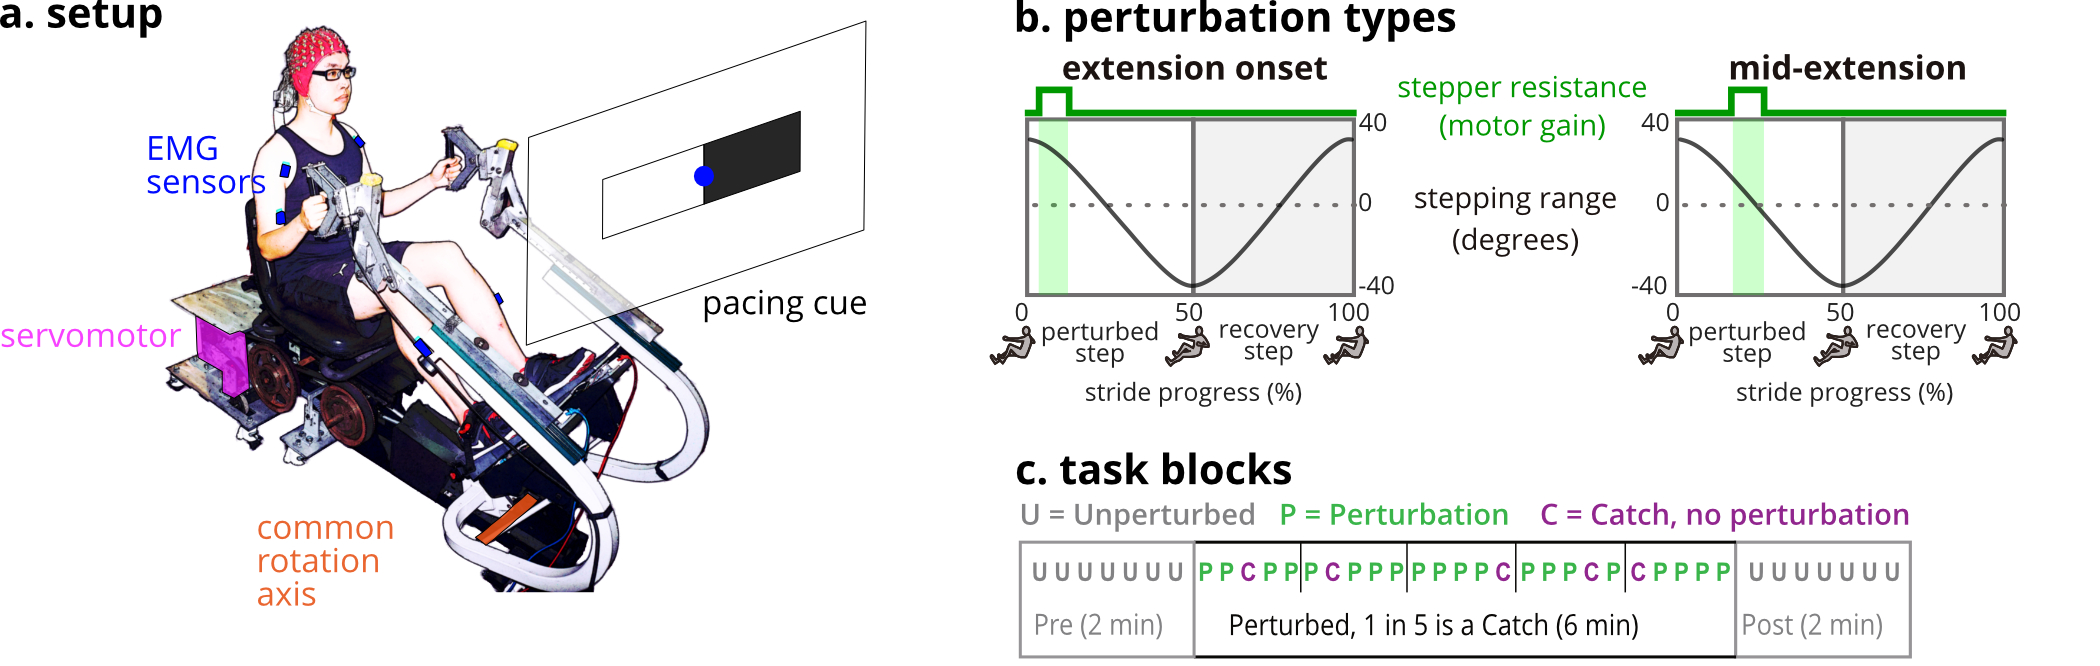
\includegraphics[width=\linewidth]{../img/01_device_protocol.jpg}
      \caption{Schematic of the robotic recumbent stepper, perturbations types, and stepping blocks. \textbf{a.} The robotic recumbent stepper is a one-degree-of-freedom stepping device with an integrated servomotor. The handles and pedals are mechanically coupled such that any limb can drive the stepping motion and move all of the other limbs. A pacing cue of alternating black and white rectangles that were 180 degrees out of phase with another was projects on a screen in front of the subject.  \textbf{b.} Perturbations were brief increases in stepping resistance in the extension-onset or mid-extension of each stride (shaded light green vertical rectangle). \textbf{c.} Each task block consisted of six minutes of perturbed stepping padded by two minutes of unperturbed stepping at the beginning and end of the task. Random catch strides did not include a perturbation.}
      \label{fig:device}
\end{figure}

\subsection{Protocol}
Data collection started with two minutes of quiet sitting, was followed by four 10-minute stepping \underline{tasks}, and ended with another two minutes of quiet sitting. Each stepping task only included one \underline{type} of perturbation, i.e., two perturbation windows (extension-onset or the mid-extension) x two legs = four perturbation type. The order of the perturbed trials was pseudorandomized. Each perturbed stepping task included three different \underline{blocks} (Figure \ref{fig:device}c): 1) \textbf{pre}: two minutes of unperturbed stepping at the start of each trial. 2) \textbf{perturbed stepping}: six minutes of perturbed strides with a single perturbation type. 3) \textbf{post}: two minutes of unperturbed stepping immediately after the end of the perturbed stepping period.  The perturbed stepping block also included a random ``catch" stride in every five perturbed strides, which did not apply a perturbation. We use pre and pre-perturbation interchangeably and also use post and post-perturbation interchangeably.

We strapped the subject's feet on the pedals, adjusted the seat position, and moved the handles to ensure subjects would not lock their knees and could drive the stepper with the handles easily. Before each task, we instructed the subjects to \textbf{A)} step smoothly as if they were walking, \textbf{B)} use both their arms and legs to drive the stepper, and \textbf{C)} follow the pacing cues that were projected in front of them (Figure \ref{fig:device}). Pacing cues were set at 60 steps per minute to match older adults' average walking pace \cite{Tudor-Locke2018-gl} and were projected as two reciprocating black and white rectangles (Figure \ref{fig:device}). We did not provide any instruction on how to interpret the pacing cues. Subjects were given at least two minutes of training to become familiar with the pacing cues before starting the data collection.

\subsection{Stepping preprocessing and stride events}
We separated each task into blocks and strides after importing the stepping data into MATLAB. We defined a stride as the time from one extension-onset of the perturbed leg to the next extension-onset of the perturbed leg for each task. For each stride, we identified the following \underline{events}: perturbed-leg extension onset, perturbation (start time), unperturbed-leg extension onset, and the end of the stride. We artificially inserted perturbation events to the unperturbed strides (i.e., pre, post, and catch strides), at the average latency the perturbation events during the perturbed strides. We excluded any incomplete strides, which were strides that did not include all the events.

\subsection{Motor Errors}
We quantified two motor error metrics, one temporal and one spatial, from the stepping kinematics. Based on the pacing cues at 60 steps-per-minute, subjects should have completed each stride in two seconds. We defined temporal error as the stride duration error, which was the difference between each stride duration and the two seconds (Figure \ref{fig:errorm}a). Because we instructed subjects to step smoothly, we expected the stepping profiles to be smooth and rhythmic during the pre-perturbation block. We defined spatial error as a stepping position error, i.e., the maximum difference of the time-normalized position profile during each stride from the averaged pre-perturbation stepping profile (Figure \ref{fig:errorm}b).

\subsection{EMG processing}
We imported and analyzed the EMG data in the Python environment using a custom processing pipeline based on Banks et al. \cite{Banks2017-dn}. We resampled the EMG data to 1 kHz, band-pass filtered between 30 and 200 Hz, rectified, and low-pass filtered at 20 Hz to obtain the EMG linear envelopes. Filters were designed using the 6th-order Butterworth algorithm. We chose 20 Hz as the low-pass threshold to capture EMG fluctuations in response to our 200-ms perturbations \cite{Shiavi1998-vu}. We then epoched and time-normalized the EMG data based on the stepping events for each stride. Finally, we normalized each muscle's linear envelope to the overall average of the muscle's linear envelope across all tasks.

\begin{table}[H]
    \centering
    \caption{Agonist muscles to drive the stepper for the left- and right-side tasks. L = left. R = right.}
    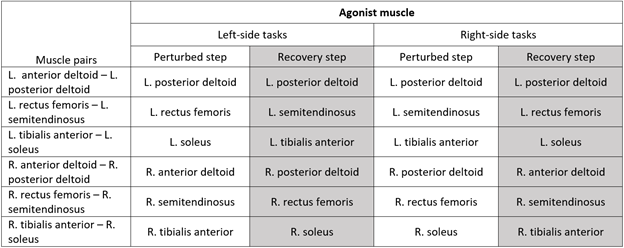
\includegraphics{../img/agonist.png}
    \label{tab:agonist}
\end{table}

We used the 'fixed' approach to quantify co-contraction \cite{Banks2017-dn}. We assumed that the agonist was the muscle that could drive the stepper without the activity of the other muscles. During the step that involved left leg extension, the left soleus, left rectus femoris, left posterior deltoid, right tibialis anterior, right semitendinosus, and right anterior deltoid act as functional agonists. The agonist muscles of the muscle pairs for each step are summarized in Table 1. The fixed co-contraction index (CI) is calculated using the following equation:

\[CI=\frac{2*I_{antagonist}}{I_{agonist}+I_{antagonist}}\]

Here, I\tsu{antagonist} and I\tsu{agonist} are the integrals of the EMG linear envelopes over each step. Because of the stepper's inherent redundancy, subjects may use a subset of agonists to drive the stepper and use a few antagonist muscles to control stepping. CI is usually expected to remain <1, so the net activity of the muscle pair can drive the limb in the designated stepping direction. However, in our study, CI might become >1 if the designated antagonist helps to control stepping while the agonist is not involved in driving the stepper. CI <1 means that the muscle pair is mainly driving the stepping motion; CI >1 would mean that the muscle pair is resisting the motion; and CI \td1 means that the muscle pair either controls the motion or is not active.

\subsection{Statistical Analysis}
The motor errors, mean EMG, and co-contraction indices have a single value per stride (or step) for each subject. We used the SMART toolbox to report the errors and co-contraction values as continuous variables (van Leeuwen et al., 2019). The main advantages of using SMART over binning methods are that each subject contributes equally to the overall average and that the comparisons benefit from multiple-comparison correction and increased statistical power.
\begin{figure}[bt]
    \centering
    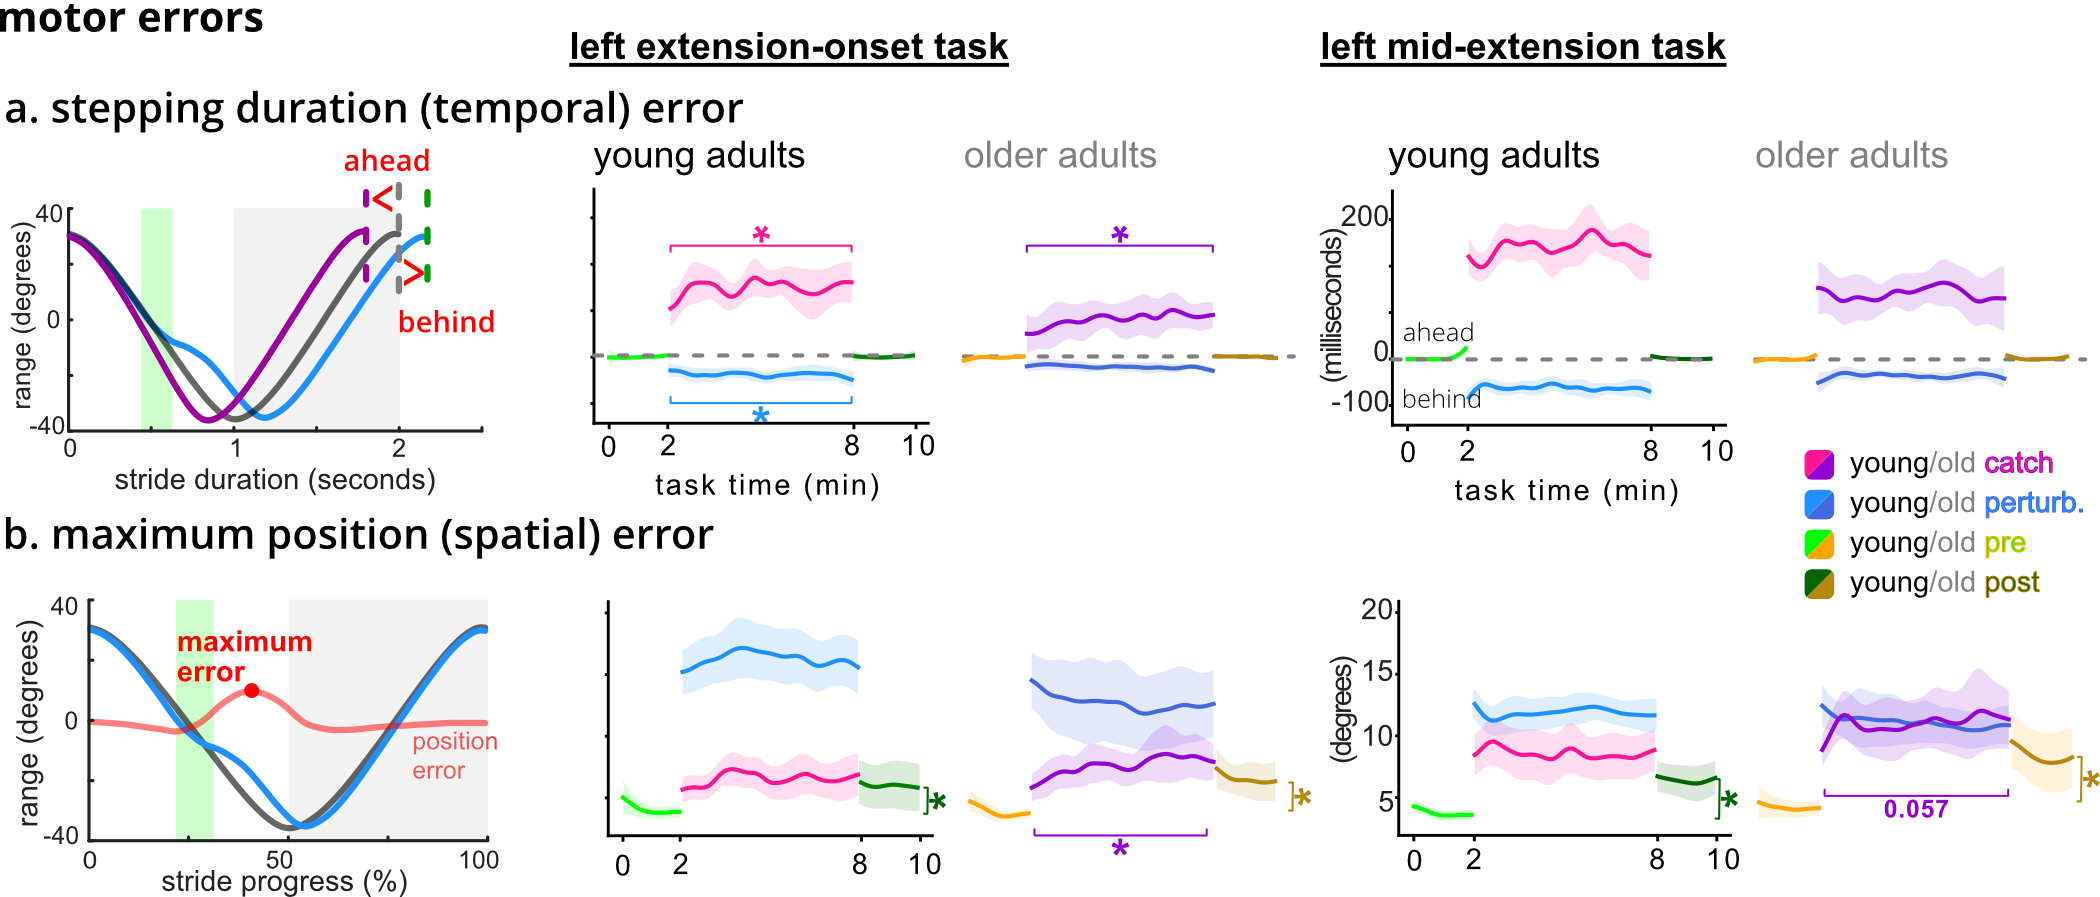
\includegraphics[width=\linewidth]{../img/02_error-metrics.jpg}
    \caption{Schematic of motor errors and the motor error behavior for the left extension-onset and left mid-extension task blocks for young and older adults. For the far-left column, the vertical shaded light green rectangles indicate the period of the perturbations while the gray shaded box highlights the recovery step. The thick lines in the time courses are the mean and the shaded areas are the confidence intervals. * p<0.05. Horizontal brackets indicate significant differences from start to end. Vertical brackets indicate significant differences between end of pre and end of post. \textbf{a.} The stepping duration (temporal) error was the difference between the duration of each step and the two-second mark set by the pacing cue (gray line). Young and older adults could maintain their temporal errors <100ms during the perturbed strides. \textbf{b.} The maximum position (spatial) error was the maximum difference between each stride’s profile and the average baseline (pre) stepping profile. Spatial errors for young adults for the perturbed and catch strides did not converge by the end of the perturbation period whereas there was convergence for the older adults. Young and older adults sustained the increased spatial errors after the perturbations were removed during post (8-10 minutes) for both perturbation types.}
    \label{fig:errorm}
\end{figure}

We used the Pingouin toolbox version 0.3.10 for our statistical analysis (Vallat, 2018). We compared motor errors, mean EMG, and co-contraction indices for each task at the end of pre, and the start and end of perturbed, catch, and post-perturbation blocks using repeated-measure analysis of variance (rANOVA). If the rANOVA was significant, we performed a priori post-hoc paired t-tests between the following pairs: 1) end of pre and end of the post to evaluate prolonged adaptation and sustained modifications 2) the start and end of perturbed strides to evaluate adaptation, 3) the start and end of catch strides to evaluate adaptation and anticipatory responses, 4) the start and end of the post to evaluate de-adaptation. We compared pre, and post-perturbation mean EMG and co-contraction indices between young and older adults using mixed-design ANOVA with age as the between-subject factor with two levels, young and old, and time as the within-subject factor, also with two levels, pre and post. We used Pingouin's {\tt pairwise-ttest} function value to 1 to determine if each muscle pair were driving (CI < 1), resisting (CI > 1), or controlling (CI ~1) the motion.with the automatic correction to perform the post-hoc tests if the mixed-design ANOVA was significant. We also compared the co-contraction index (CI) value to 1 to determine if each muscle pair were driving (CI < 1), resisting (CI > 1), or controlling (CI \td1) the motion. We used SMART's one-sample statistical test to determine if CI was different from one. The significance level of all statistical analyses was set to 0.05.

\section{Results}
\subsection{Temporal error}
Young and older adults did not reduce their temporal errors as they gained more experience with the perturbations, indicating a lack of error-based adaptation, but they did de-adapt after the perturbations were removed (Figure \ref{fig:errorm}a). Both young and older adults had ~50ms temporal errors during perturbed strides, while the temporal errors during catch strides were ~150ms (Figure \ref{fig:errorm}a). The rANOVA was significant for temporal errors in each task (young adults F\tsu{(6,96)}>40, p< 0.0005, older adults F\tsu{(6,96)}>20, p< 0.0005). However, the post-hoc a priori tests only indicated significant and meaningful differences in the left mid-extension temporal errors at start and end of catch strides for both young and older adults (young adults p=0.047, older adults p=0.025). Both young and older adults reduced their temporal errors to baseline levels after the perturbations were removed, indicating de-adaptation. The right-side showed also similar temporal errors, with the exception of young adults increasing their temporal errors form start to end of both perturbed and catch strides (F\tsu{(6,96)}=144, p< 0.0005, post hoc p<0.01) (Supplementary Figure \ref{fig:S1}a).

\subsection{Spatial error}
Spatial errors of older adults during catch and perturbed strides converged by the end of the perturbed block whereas there was no convergence for young adults (Figure \ref{fig:errorm}b). Spatial errors for young adults during the catch strides were ~10° for both perturbation tasks, which was less than ~12° for left extension-onset perturbed strides and ~16° for the left mid-extension perturbed strides. However, the difference between the spatial errors of catch strides and of perturbed strides for older adults was not present in the left extension onset and diminished toward the end of the left mid-extension perturbations. The rANOVAs were significant for the spatial errors of every task (young adults F\tsu{(6,96)}>20, p< 0.0005, older adults F\tsu{(6,96)}>10, p< 0.0005). The post-hoc tests showed that the spatial errors for older adults were different from the start to the end of the catch strides for both left extension-onset and left mid-extension tasks (extension-onset p = 0.023, mid-extension p = 0.057).  After removing the perturbations, spatial errors were always higher than pre levels for both young and older adults and did not return to pre levels (post hoc, young adults: extension-onset p=0.018, mid-extension p=0.001; older adults: extension-onset p=0.008, mid-extension p=0.009). For the right side tasks, spatial errors of catch strides for older adults did not increase from start to end (Supplementary Figure \ref{fig:S1}b). Nevertheless, spatial errors were also higher during the right-side task’s post blocks than the pre, but older adults (post hoc, young adults' extension-onset p=0.001, mid-extension p<0.0005, older adults' extension-onset p=0.005, mid-extension p=0.002).

\subsection{Muscle activity and co-contraction for the extension-onset perturbation tasks}
Young and older adults used their left (ipsilateral) rectus femoris and right (contralateral) anterior deltoid to drive the stepper during the left extension-onset perturbed steps (Figure \ref{fig:LEIEMG}). The agonist muscles (e.g., left rectus femoris and right anterior deltoid) were active mainly during the extension-onset, and the antagonist muscles (e.g., left semitendinosus and right rectus femoris) became active toward the end of the step, likely to slow down the stepping motion and assist with a smooth transition between steps (Figure \ref{fig:LEIEMG}, EMG profile). Of the six agonist muscles that young and older adults could use to drive the stepper, the left rectus femoris and the right anterior deltoid showed greater muscle activity during perturbed strides than catch strides (Figure \ref{fig:LEIEMG}, EMG mean). The mean left posterior deltoid antagonist activity increased during the recovery steps for young adults and did not return to the pre-perturbation levels after removing the perturbations (rANOVA F\tsu{(6,96)}=2.4, p=0.01, post-hoc perturbed stride p=0.06, pre-post p=0.03). Older adults, however, showed greater mean EMG at the end of the post block compared to pre block for the left anterior deltoid, right anterior deltoid, and right soleus (rANOVA F\tsu{(6,60)}'s>3.0, p's <0.01, post hoc p's <0.05). Simialr to the left side, right recuts femoris were active during the perturbaed strides (Supplementary Figure \ref{fig:S2}). While most muscles ahd slightly increased their mean EMG, the right anterior deltoid mean EMG decreased for young adults during both perturbed and recovery steps and for older adults during the recovery step (rANOVA F\tsu{(6,60)}'s>3.5, p's <0.01, post hoc p's <0.05).

During the perturbed steps of the left extension-onset task, young adults only had CI \td1 for their right tibialis anterior-soleus while CIs for the other muscle pairs were <1 (SMART p’s<0.05) (Figure \ref{fig:LEIEMG}, co-contraction index). During the recovery steps, CIs for left anterior deltoid-posterior deltoid and right anterior deltoid-posterior deltoid were \td1. Older adults, however, had CIs \td1 for all muscle pairs except for the left and right rectus femoris-semitendinosus during the perturbed step and left tibialis anterior-soleus during the recovery steps (SMART p’s<0.05). Older adults reduced their co-contraction during the perturbation block for the left rectus femoris-soleus while using their right anterior deltoid-right posterior deltoid pair to resist the motion during the recovery steps (SMART p’s<0.05). For the right extension-onset task, older adults also demonstrated similar CI reduction for the left anterior deltoid-posterior deltoid and briefly for the right rectus femoris-semitendinosus and the left and right tibialis anterior-soleus (Supplementary Figure \ref{fig:S2}).

\begin{figure}[H]
    \centering
    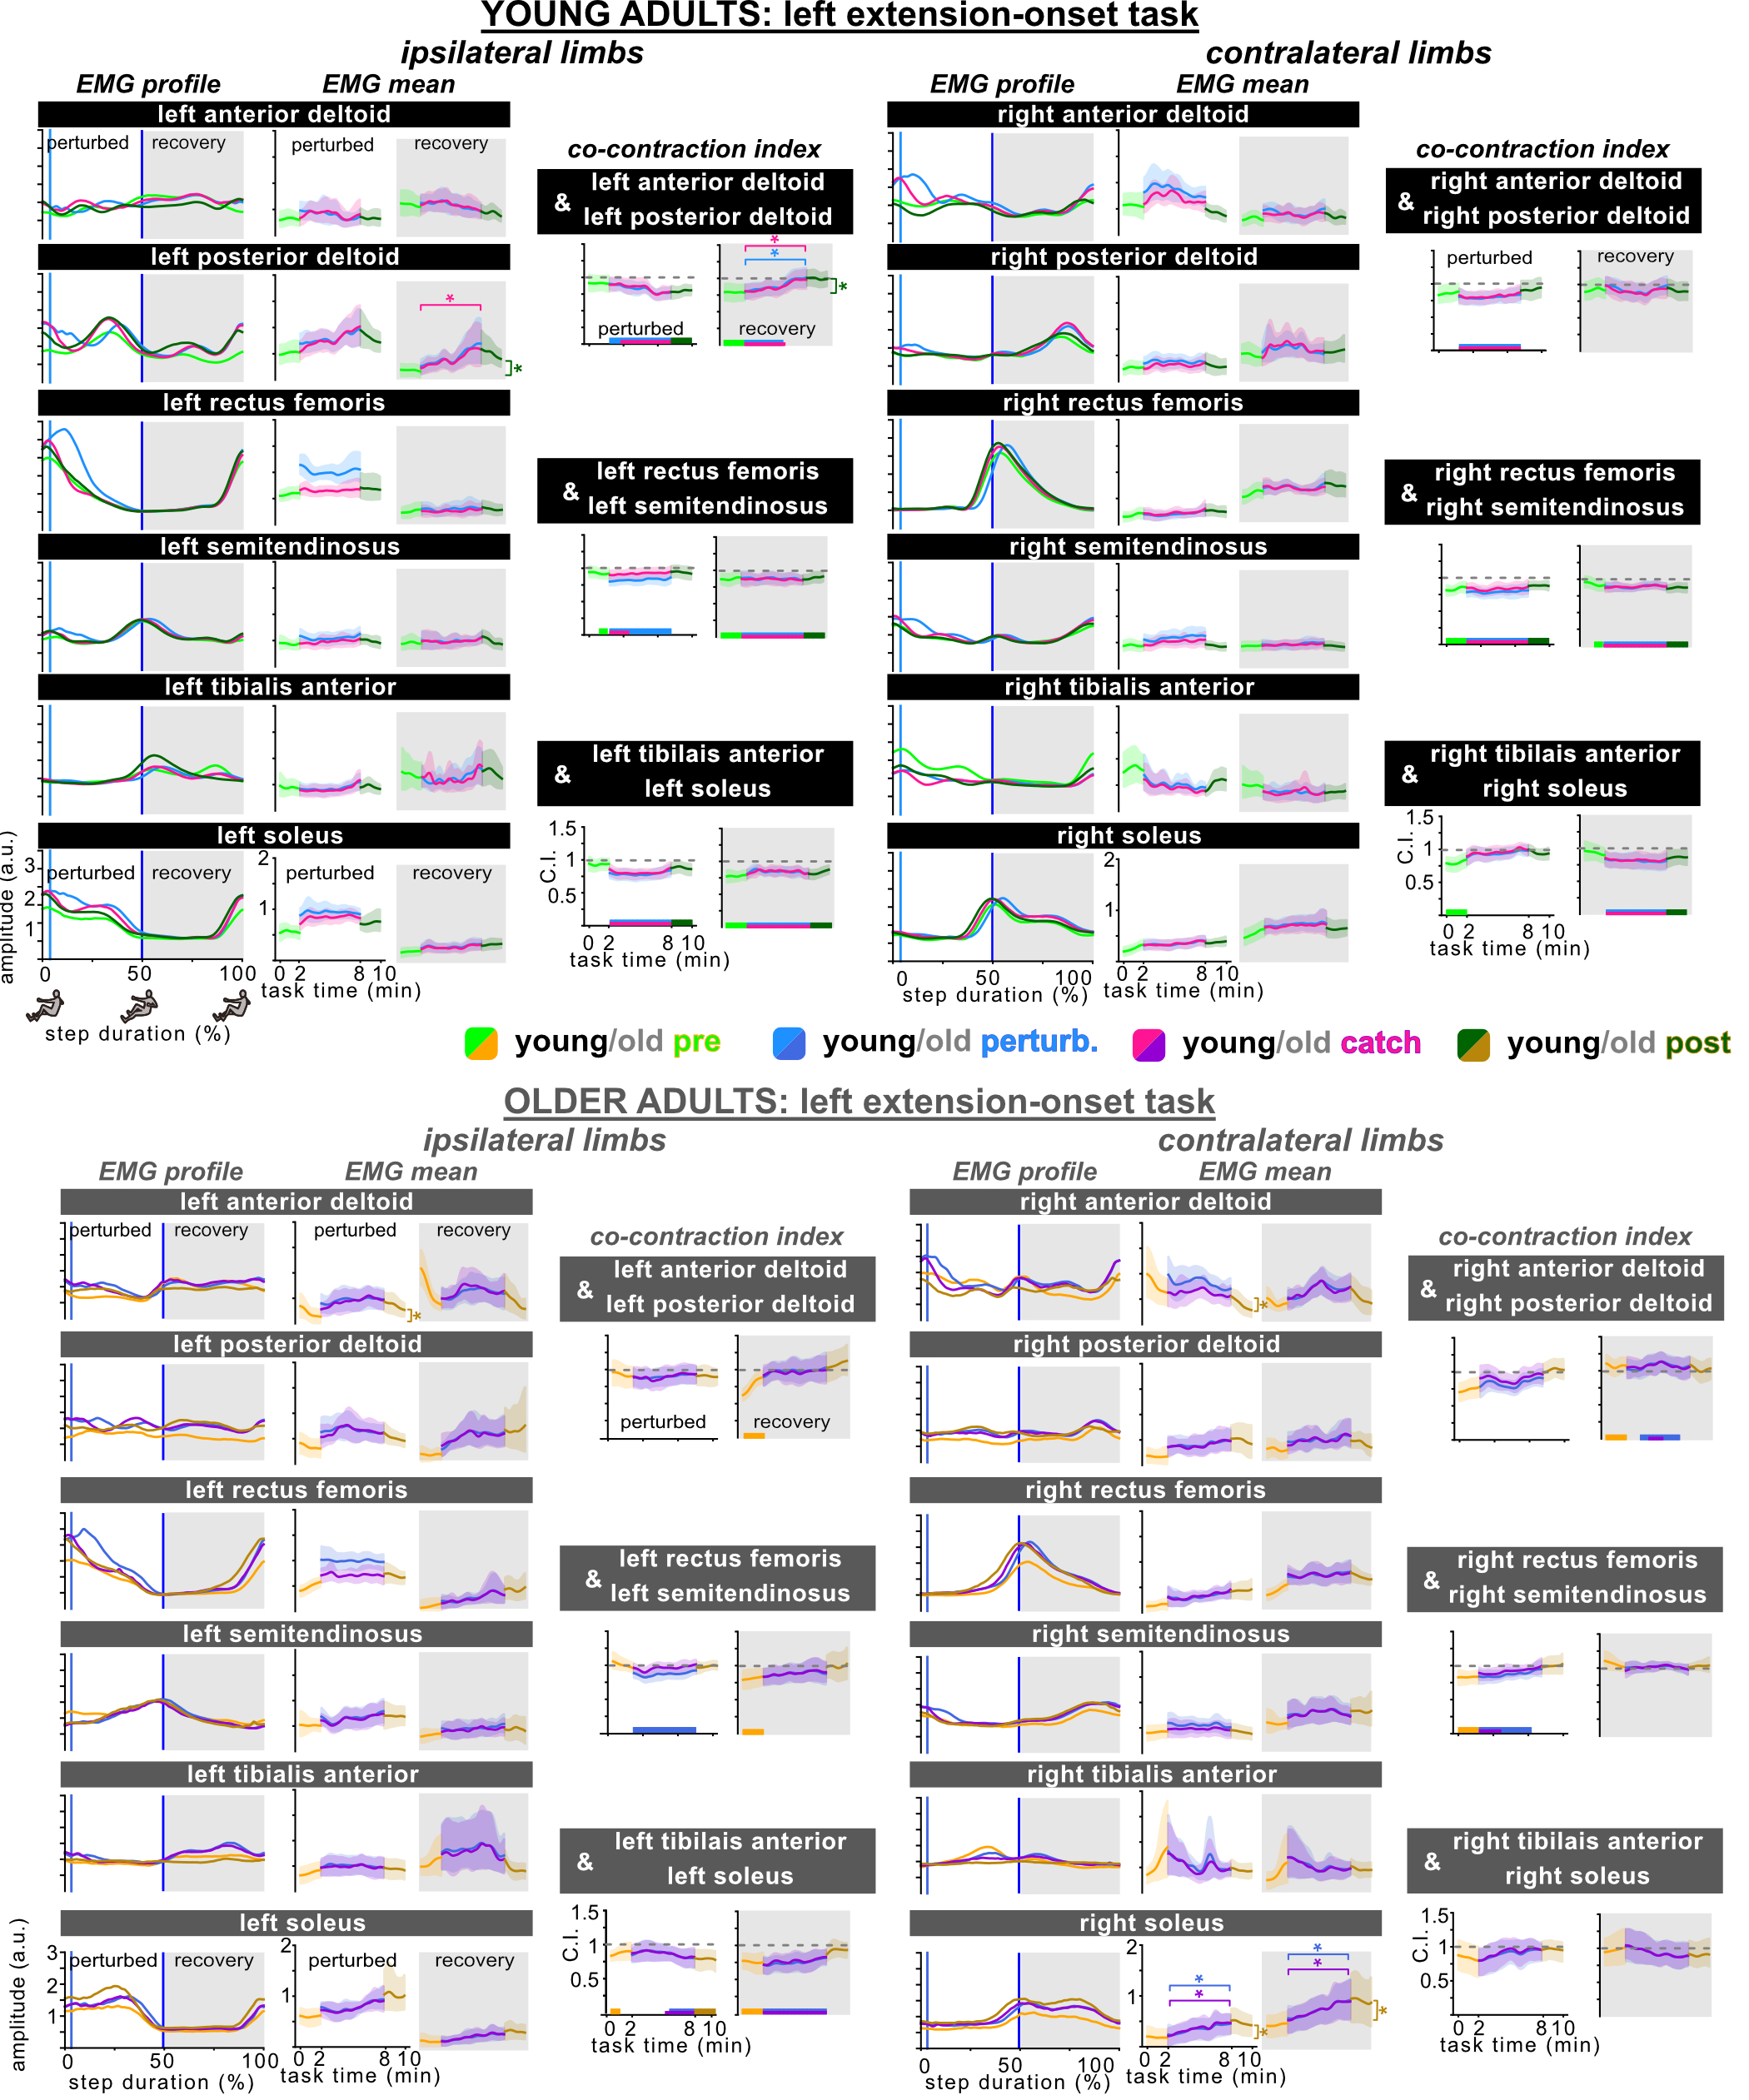
\includegraphics[scale=.8]{../img/03_LEI-EMG-CoCont.jpg}
    \caption{EMG profiles (i.e. linear envelopes), time course of the EMG means for each block, and the time course co-contraction indices for the \textbf{left extension-onset} task for young (black headers) and older (gray headers) adults. The EMG profile is the grand average across the strides and subjects within the age-group. EMG mean and co-contraction is quantified per each perturbed and recovery step for the duration of the task.  In the time courses, the thick lines are the mean and the shaded regions are the confidence intervals. * indicates significant post-hoc test. Colored rectangles at the bottom of the co-contraction plots indicate difference from 1 using SMART.}
    \label{fig:LEIEMG}
\end{figure}

\subsection{Muscle activity and co-contraction for the mid-extension perturbation tasks}
Young adults used a greater number of agonists during left mid-extension than older adults (Figure \ref{fig:LMEEMG}). Young adults used the left (ipsilateral) posterior deltoid, left rectus femoris, left soleus, right (contralateral) semitendinosus, and right tibialis anterior to drive the stepper during the perturbed step (Figure \ref{fig:LMEEMG}, EMG profile). The antagonist muscle activity was dominant toward the end of the perturbed step, similar to the left extension-onset task. The left mid-extension perturbations resulted in increased left soleus activity for young adults during perturbed and recovery steps even after the perturbation was removed (rANOVA F’\tsu{(6,96)}s>2.3, p’s<0.03, post hoc p’s<0.05). Older adults used their left posterior deltoid, left rectus femoris, left soleus as agonists to overcome the left mid-extension perturbations (Figure \ref{fig:LMEEMG}, EMG profile). During the left mid-extension perturbation task, right and left rectus femoris and left posterior deltoid EMG activity significantly increased for older adults irrespective of their role in the movement (rANOVA F\tsu{(6,54)}'s>4.3, p's <0.001, post hoc p's <0.05) (Figure \ref{fig:LMEEMG}, EMG mean). Young and older adults used largely the same muscles to overcome the right mid-extension perturbations, namely right (ipsilateral) posterior deltoid, left rectus femoris, right (contralateral) anterior deltoid. Older adults also continuously used their right soleus to drive the stepper which resulted increase in mean EMG for the perturbed and recovery steps during perturbed stride and form pre to post (rANOVA F\tsu{(6,60)}'s>2.3, p's <0.04, post hoc p's <0.05) (Supplementary Figure \ref{fig:S3}).

The older adults had a significant CI increase during the perturbed step for the right anterior deltoid-posterior deltoid pair due to the increased antagonist right posterior deltoid became activity right after the perturbation (Figure \ref{fig:LMEEMG}, EMG profile; CI rANOVA F\tsu{(6,54)}=4.0, p=0.002, post hoc p’s<0.01). Like the left extension-onset tasks, the Cis for muscle pair in young adults were <1 except for the anterior deltoid-posterior deltoids during the perturbation block (SMART p’s<0.05). Older adults significantly reduced their CI during the perturbation block in the left anterior deltoid-posterior deltoid, left rectus femoris-semitendinosus, and the right tibialis anterior-soleus to help drive the perturbed step (SMART p’s<0.05). For the right mid-extension task, older adults demonstrated a similar CI reduction for the right and left anterior deltoid-posterior deltoid, briefly for the left rectus femoris-semitendinosus, and the left and right tibialis anterior-soleus (Supplementary Figure \ref{fig:S3}).

\subsection{Muscle activity and co-contraction differences pre to post for the extension-onset tasks}
Overall, more muscles had significantly different amplitudes from pre to post in the left extension-onset taskthan the left mid-extension perturbations (Figure \ref{fig:lpp}). The left posterior deltoid showed the most significant  differences between young and older adults and the pre and post blocks during the left extension-onset task (mixed-design ANOVA F\tsu{(1,26)}'s>5, P's <0.03, post-hoc, pre-post p's<0.03). The mean EMG increased and was sustained from pre to post for the left posterior deltoid for both perturbed and recovery steps, and the mean EMG for young and older adults was also different in the perturbed (left) step (mixed-design ANOVA F\tsu{(1,26)}'s>4, p's <0.03, post-hoc, pre-post p's <0.01, age perturbed step p=0.02). These differences, however, only resulted in a significant CI increase from pre to post for the recovery steps in the left anterior deltoid-posterior deltoid in the left extension-onset task (Figure \ref{fig:lpp}, co-contraction index). During the left extension-onset task, the left and right rectus femoris, semitendinosus, and soleus showed significantly greater mean EMG during the post block compared to pre block only when they were acting as antagonists (mixed-design ANOVA F\tsu{(1,26)}'s>4, P's <0.03, post-hoc, pre-post p's<0.05). As a result, post-perturbation CI was greater than pre CI for just the right rectus femoris-semitendinosus and right tibialis anterior-soleus pairs during the perturbed (left) step (mixed-design ANOVA F\tsu{(1,24)}'s>4, P's <0.04, post-hoc, pre-post p's,<0.04). Older adults had significantly higher CI than young adults in pre and post blocks for the right rectus femoris-semitendinosus pair in the left extension-onset task (mixed-design ANOVA F\tsu{(1,26)}=7.3, P=0.01, post hoc, age effect p=0.01, age x pre p=0.06, age x post p=0.02) (Figure \ref{fig:lpp}, co-contraction index).

\begin{figure}[H]
    \centering
    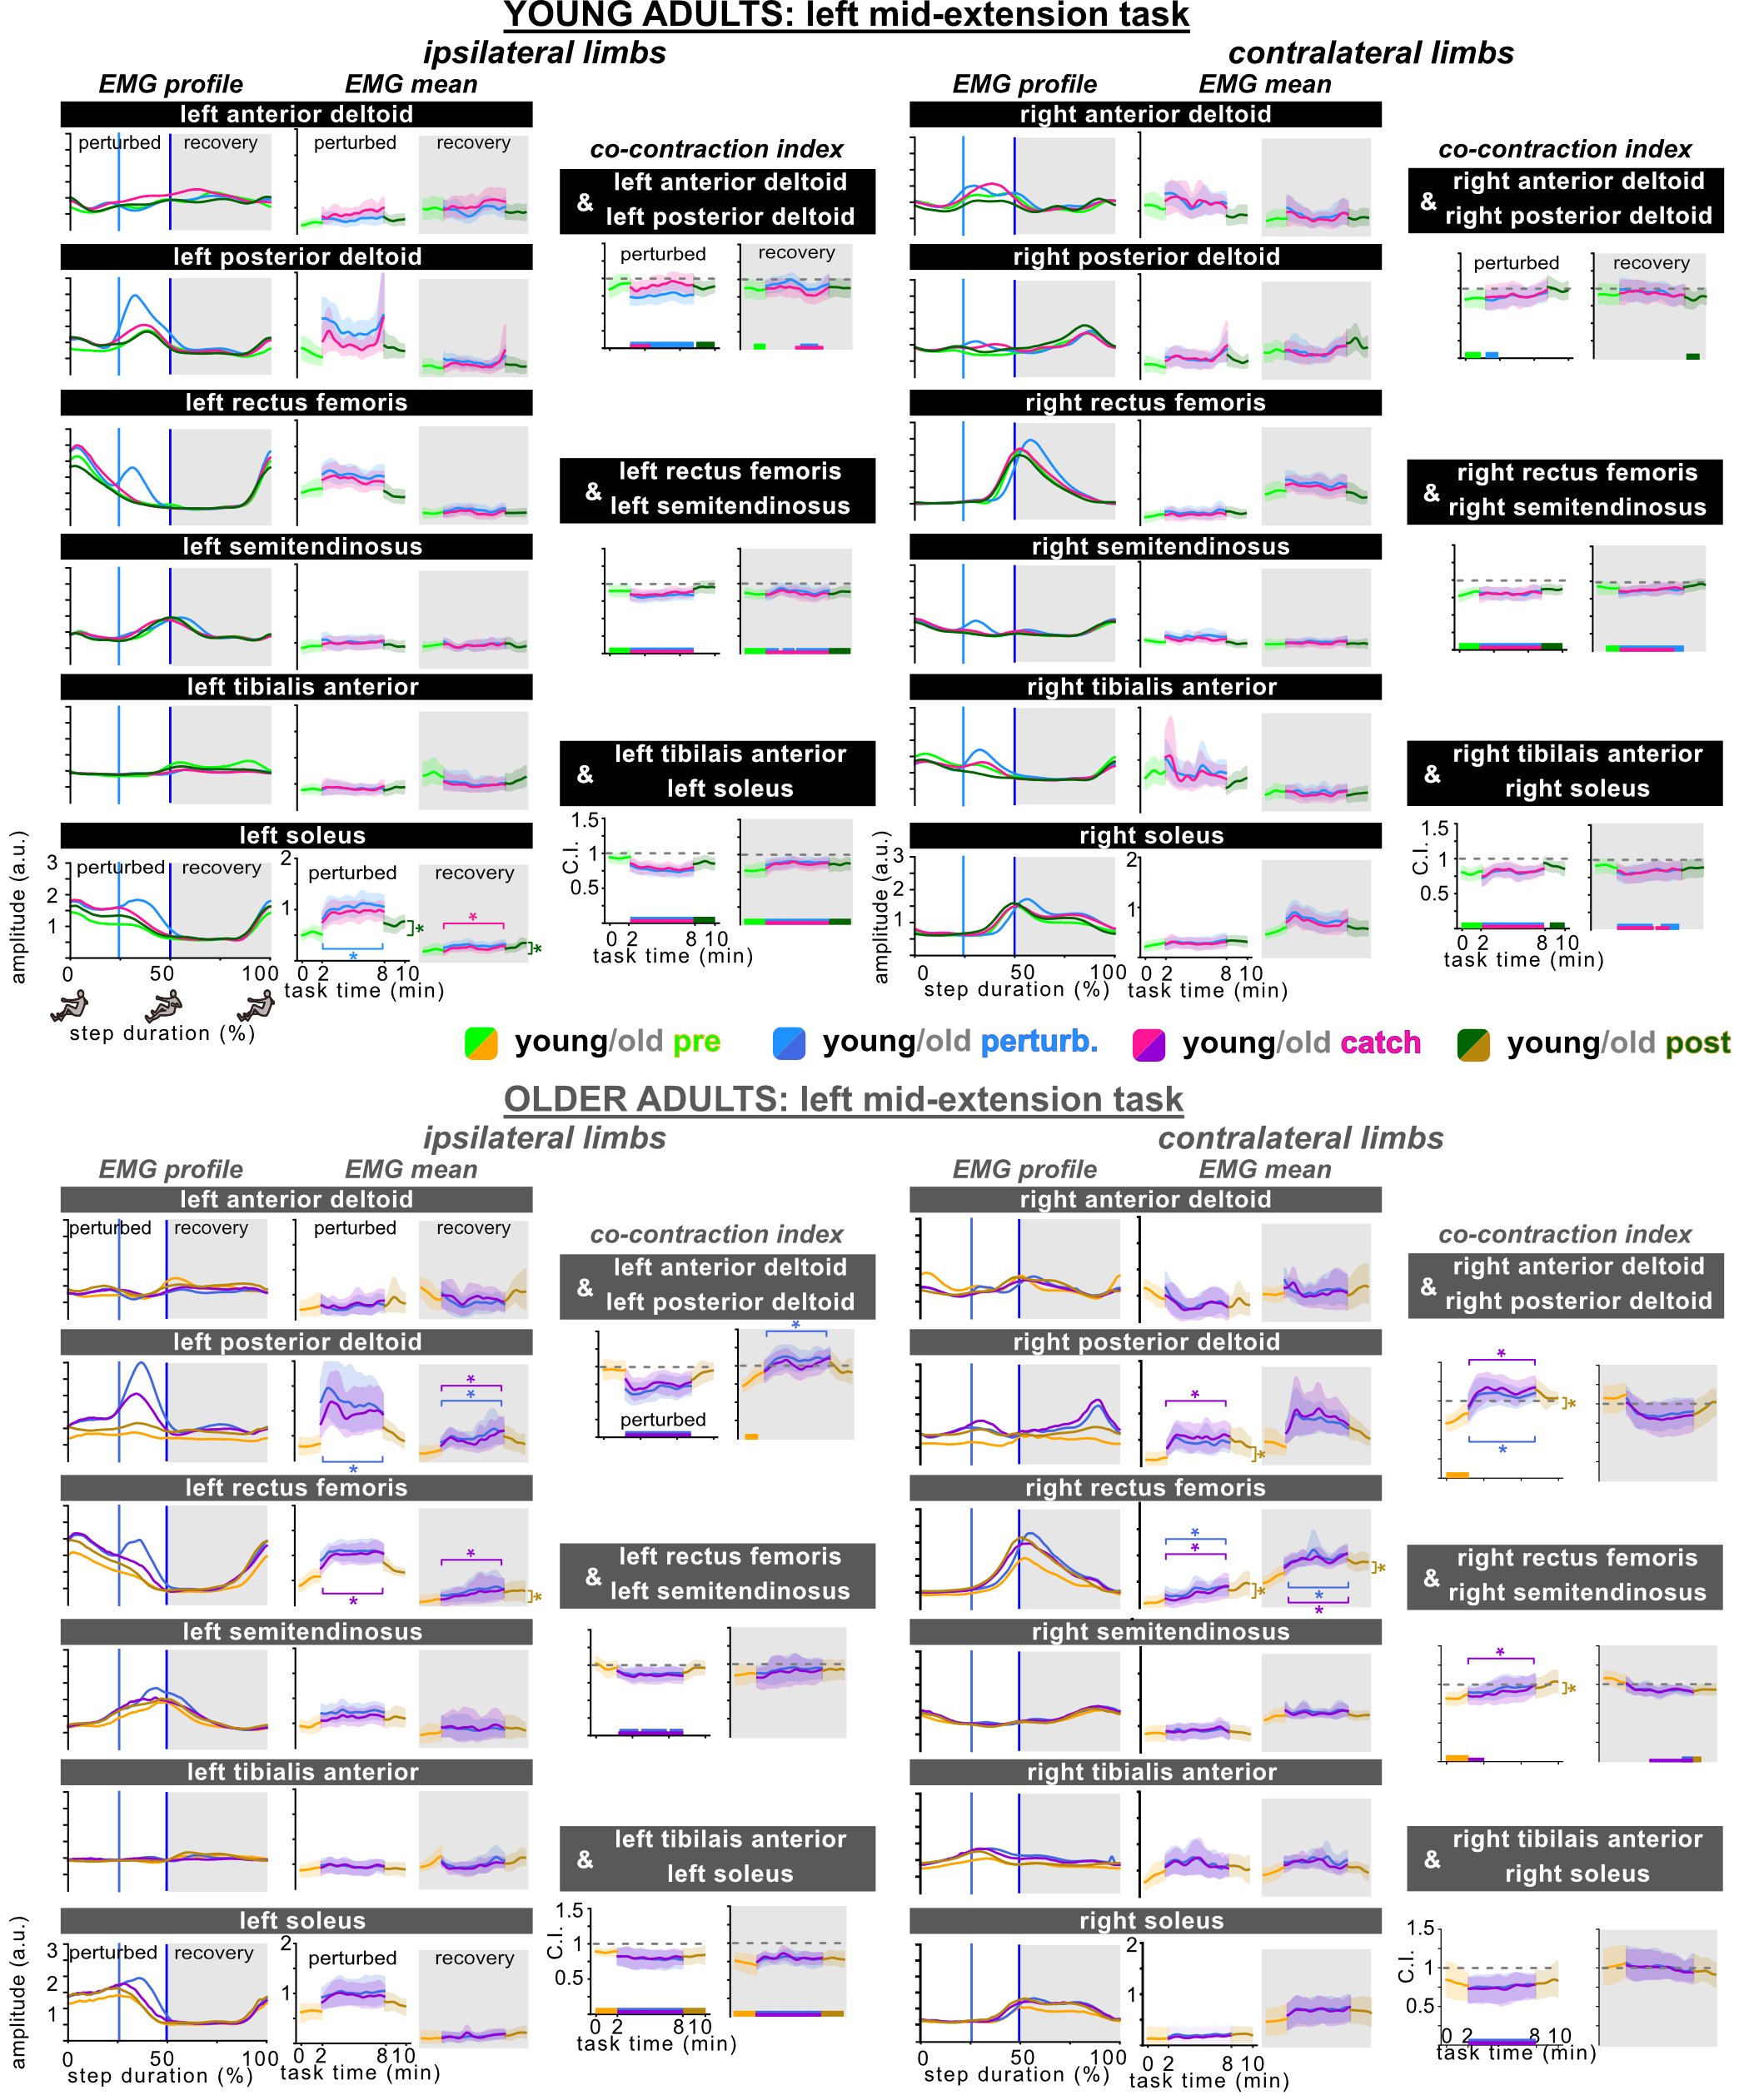
\includegraphics[scale=.8]{../img/04_LME-EMG-CoCont.jpg}
    \caption{EMG profiles (i.e., linear envelopes), time course of the EMG means for each block, and the time course co-contraction indices for the \textbf{left mid-extension task} for young (black headers) and older (gray headers) adults. The EMG profile is the grand average across the strides and subjects within the age-group. EMG mean and co-contraction is quantified per each perturbed and recovery step for the duration of the task.  In the time courses, the thick lines are the mean and the shaded regions are the confidence intervals. * indicates significant post-hoc test. Colored rectangles at the bottom of the co-contraction plots indicate difference from 1 using SMART.}
    \label{fig:LMEEMG}
\end{figure}

\begin{figure}[H]
    \centering
    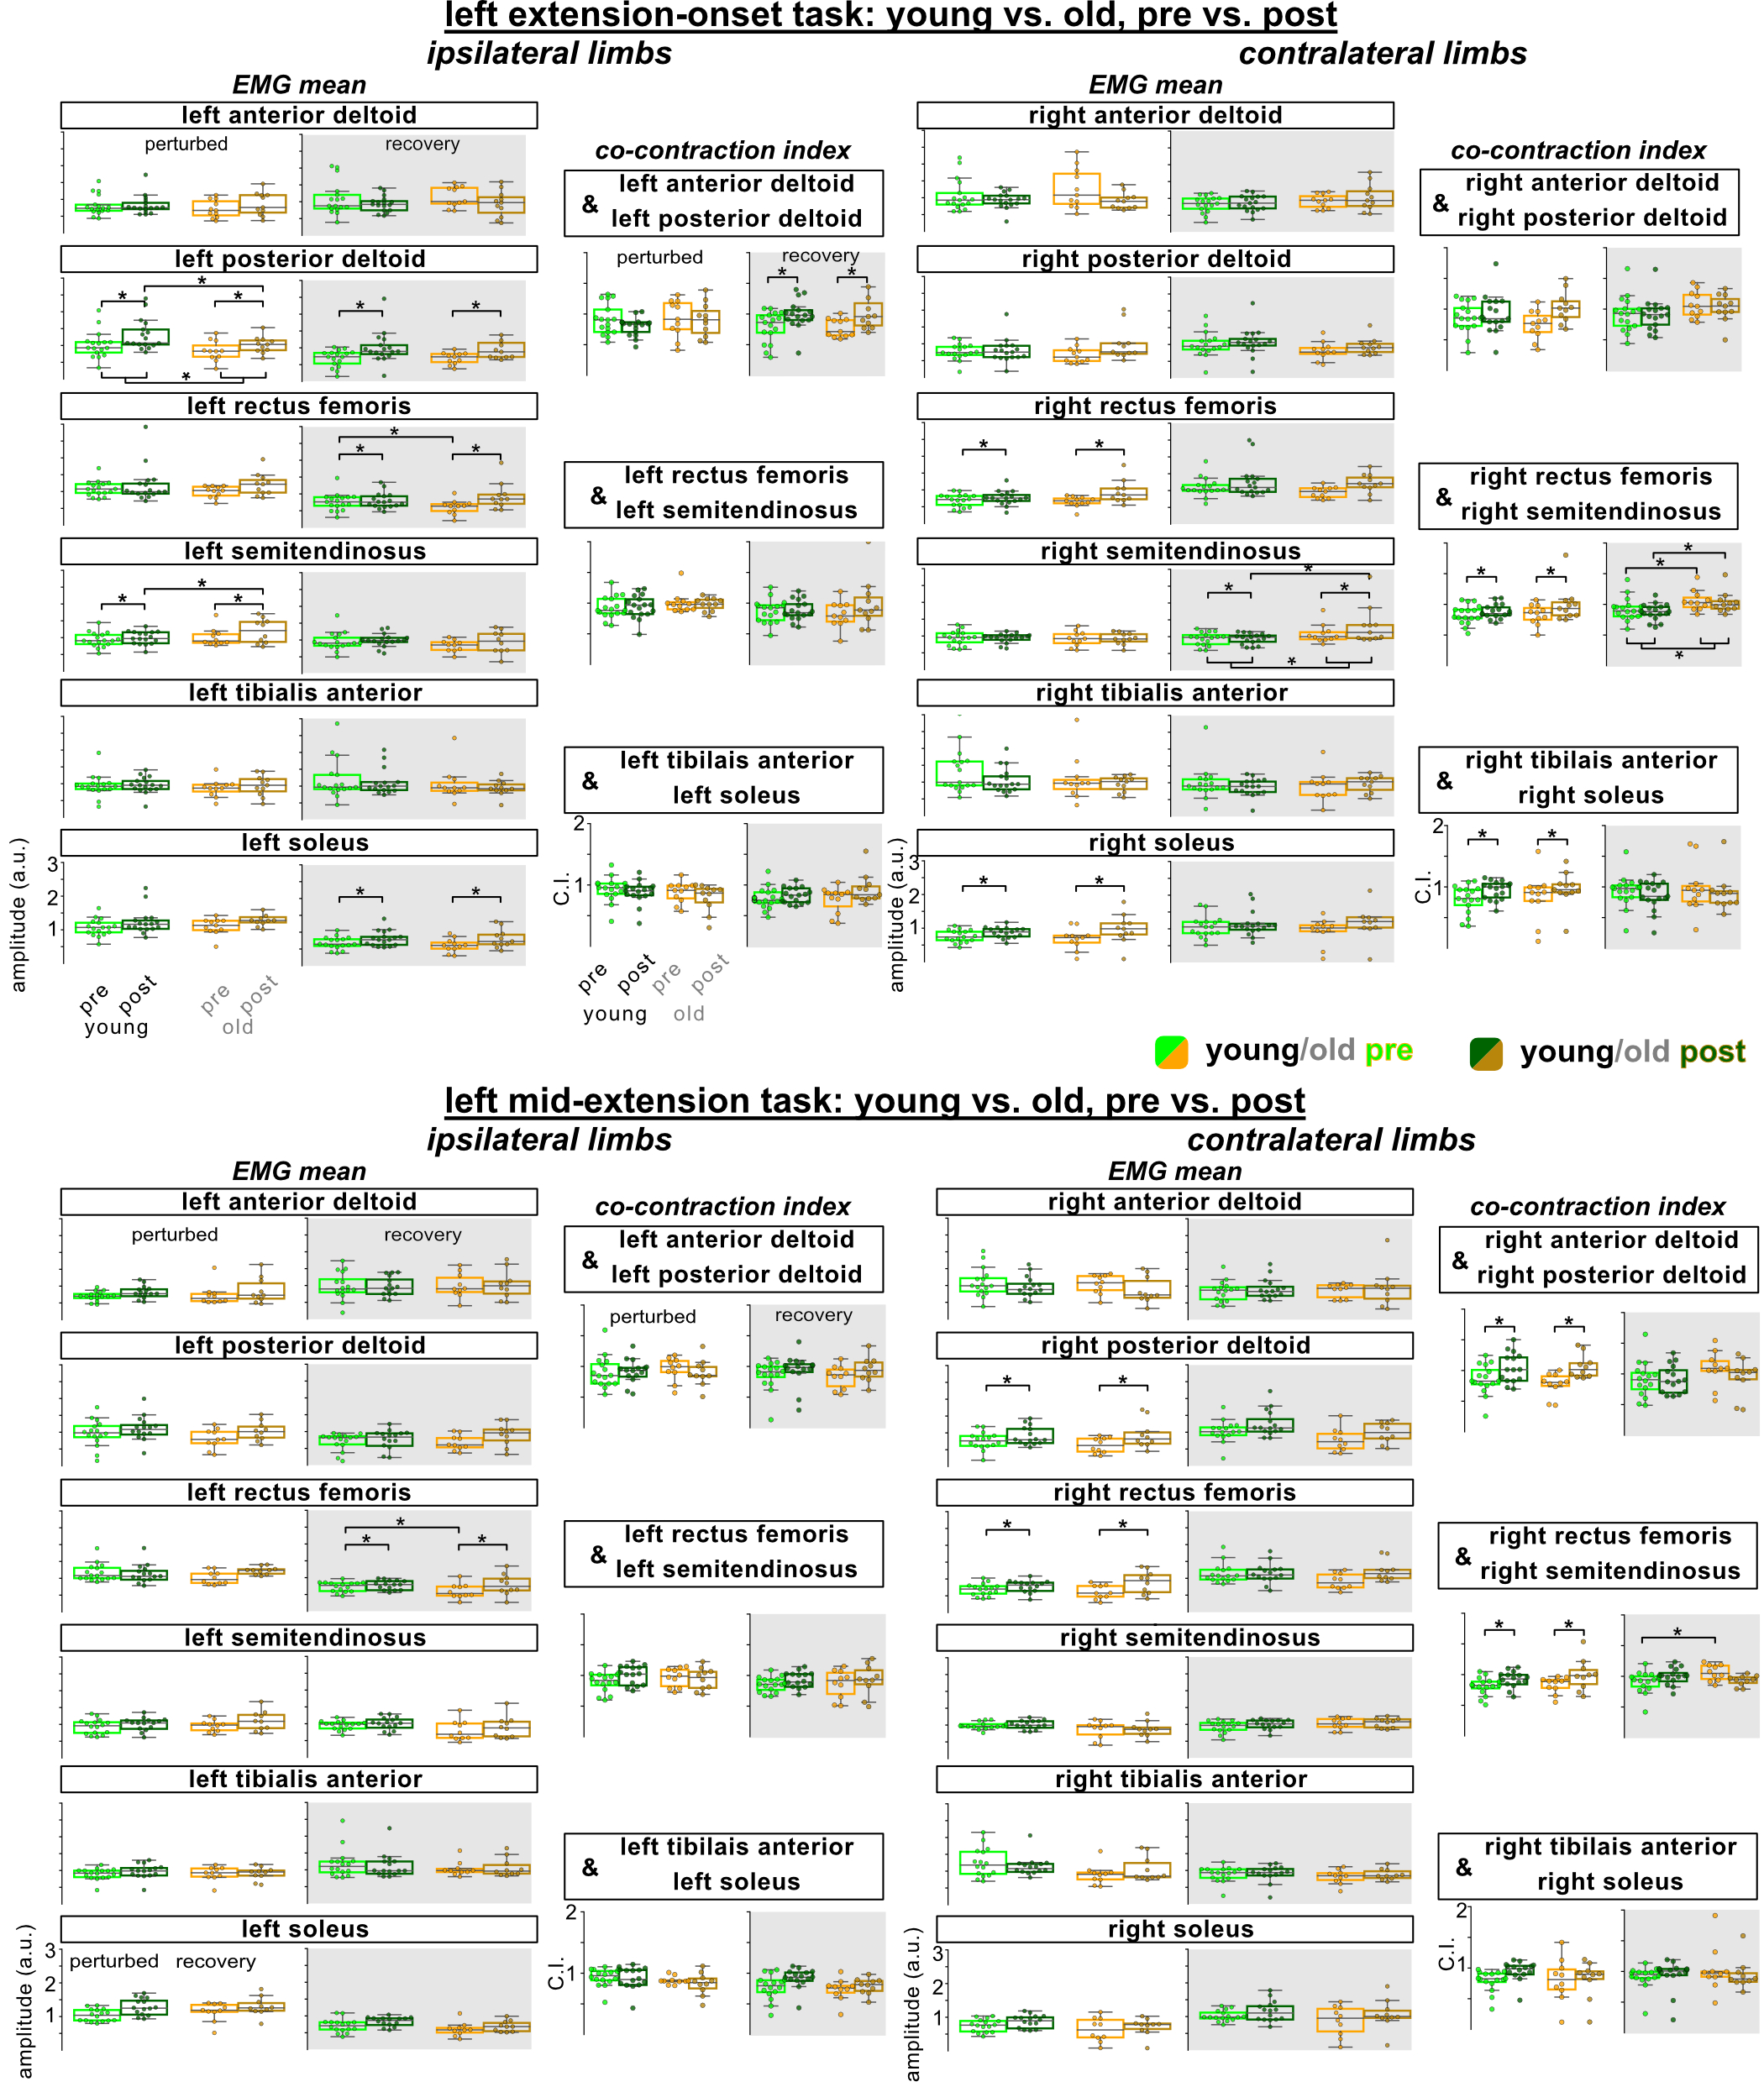
\includegraphics[scale=.8]{../img/05_pre-post-comparison.jpg}
    \caption{Comparison of mean EMG and co-contraction between pre and post for the \textbf{left-side} tasks. * indicates post hoc significant test. Boxes expand between the first and third quartile. Whiskers are minimum and maximum after rejecting the outliers. Outlier rejection is only for representation and was not included in the statistical analysis.}
    \label{fig:lpp}
\end{figure}

During the left mid-extension task, the left and right rectus femoris mean EMG were greater during the post block than the pre block, resulting in increased CI from pre to post for right rectus femoris-semitendinosus pair (mixed-design ANOVA F\tsu{(1,24)}'s >4, p's <0.04, post hoc, pre-post p's<0.04). The right posterior deltoid had greater antagonist activity during the post perturbation block for both young and older adults during the left mid-extension task, resulting in increased CI from pre to post for the right anterior deltoid-right posterior deltoid pair (mixed-design ANOVA F\tsu{(1,24)} =1.1, p =0.001, post hoc, pre-post p=0.002). For right-side tasks, there was a main effect of time (pre-post) on the EMG amplitude and co-contraction index. Additionally, age also affected the EMG mean of several muscles, including left soleus and left semitendinosus, and the CIs of several muscle-pair, including right rectus femoris-semitendinosus (Supplementary Figure \ref{fig:S4}).

\section{Discussion}
We quantified and compared the motor error behavior, muscle activity responses, and co-contraction indices of young and older adults responding to perturbations during a seated locomotor task. Like young adults, older adults retained prolonged motor modifications after the perturbations were removed, suggesting that use-dependent learning also occurred for older adults. Unlike young adults, the spatial errors in catch and perturbed strides converged by the end of the perturbation block for older adults. Young adults used more muscle pairs than older adults to drive the stepper during the perturbed steps and the recovery steps. The co-contraction of older adults generally increased as a result of the perturbations. However, older adults could also effectively reduce their CI for select muscles and change the role of the muscle pairs from controlling to driving based on the task, such as with the left rectus femoris-semitendinosus during both left extension-onset and mid-extension perturbations. Despite the different task mechanics, the results demonstrate that perturbing the stepping patterns of older adults could promote a reduction of co-contraction for select muscle-pairs based on the perturbation timing.

Use-dependent learning was clearly evident during these perturbation tasks in young and older adults, based on not just motor error behavior but also muscle activity and co-contraction indices. For young and older adults, motor errors did not decrease during the perturbed block, indicating that error-based adaptation did not occur. Instead of decreasing, the spatial errors were prolonged during the perturbed block and sustained through the post block in both young and older adults, which is indicative of use-dependent learning. This suggests that regardless of age, subjects perceived that following the pacing cue was their main goal in the perturbed stepping tasks and that modifying the stepping profile did not hinder achieving the task goal, which led to the retention of the modified stepping profile \cite{Diedrichsen2010-as}. In general for young and older adults, muscle activity was higher during the post block after the perturbations were removed compared to the pre block, which provides more evidence of use-dependent learning. Further, the co-contraction indices did not decrease as subjects gained more experience with our perturbations or from pre to post. In typical error-based adaptation studies, co-contraction often decreases with adaptation \cite{Thoroughman1999-pz,Darainy2008-li}. Taken altogether, motor errors, muscle activity, and co-contraction indices clearly indicate that use-dependent learning occurred as subjects responded to perturbations applied on a stride-by-stride basis during recumbent stepping.

Older adults used fewer muscle pairs to drive the stepper compared to young adults. Recumbent stepping is a mechanically redundant task. As such, subjects can drive the stepper with just one shoulder, elbow, hip or knee flexor-extensor muscle pair such as the left rectus femoris-left semitendinous pair or with a functional agonist-antagonist such as the left and right rectus femoris muscles that would oppose each other during stepping. In this task, the co-contraction index (CI) could delineate whether a muscle pair was driving (CI < 1), controlling (CI > 1), or refining (CI \td1) the stepping motion. Based on CI < 1, older adults had 3 out of 6 muscle pairs driving the stepping motion compared to the 5 out of 6 muscle pairs for young adults, indicating that older adults used fewer resources to drive the stepper. This aligns with previous studies of perturbed walking and perturbed balance that showed that older adults used  fewer muscle synergies to respond to the perturbations than young adults \cite{Allen2018-kd,Da_Silva_Costa2020-vl}. Overall, by increasing co-contraction to potentially increase limb stiffness, older adults seemed to be able to resist and reject the perturbations such that the older adults had similar, if not smaller, motor errors during perturbed stepping compared to young adults. The only instance of a muscle pair significantly resisting the stepping motion was during the left extension-onset perturbations for the right anterior deltoid-posterior deltoid of just the older adults.

The reduction of co-contraction in select muscle pairs during perturbations is a novel aspect of this seated locomotor task. Interestingly, perturbation could decrease CI for select muscle pairs across both right- and left-side tasks (Figures \ref{fig:LEIEMG},\ref{fig:LMEEMG} and supplementary Figure \ref{fig:S2}, \ref{fig:S3}). The CI decrease is in contrast to previous walking and balance studies which reported increased co-contraction with the presence of perturbations \cite{Tang1998-jp,Nagai2012-kp,Richards2019-tz}. The perturbation timing resulted in different muscle pairs with reduced CIs for each task. This can be especially beneficial for rehabilitation, where using different perturbations during recumbent stepping would engage specific muscle-pairs to drive the locomotion. Recent studies have indicated that seated locomotor exercise significantly improves walking performance during rehabilitation \cite{Kaupp2018-ch,Zhou2018-yy}. Transferability of perturbed seated exercises to walking improvement requires further research.

Limitations of this study include not including the handles and force data and attributing the perturbations to the extending leg. The recumbent stepper is equipped with load cells for pedals and handles. However, we decided not to use the force and moment data for this study because the inertia of the device would contaminate the force data, especially during the perturbations. While we asked subjects to use both arms and feet to drive the stepper, we attributed the perturbations to the extending leg. A previous study and our preliminary tests (not reported here) showed that the lower-limb extension contributes the most to compensate for increased stepping resistance \cite{Skinner2014-cl}.

Perturbed recumbent stepping generally increased co-contraction for both young and older adults from pre to post perturbation block and from the start to the end during the perturbation block. However, based on the timing of the perturbations, older adults reduced co-contraction of select muscle pairs to help drive the stepper. This novel effect and lack of fall risk provide the potential to use perturbations in seated locomotor tasks to help older adults reduce co-contraction and improve their motor response at the same time. Still, the efficacy of perturbed sitting tasks on walking performance and the effect of different perturbation intensity and duration require further research.



% \addbibresource{{\subfix{../refs.bib}}}
\bibliographystyle{ieeetr}
\bibliography{../refs}
\newpage
\section{Supplementary figures}
\begin{figure}[H]
    \centering
    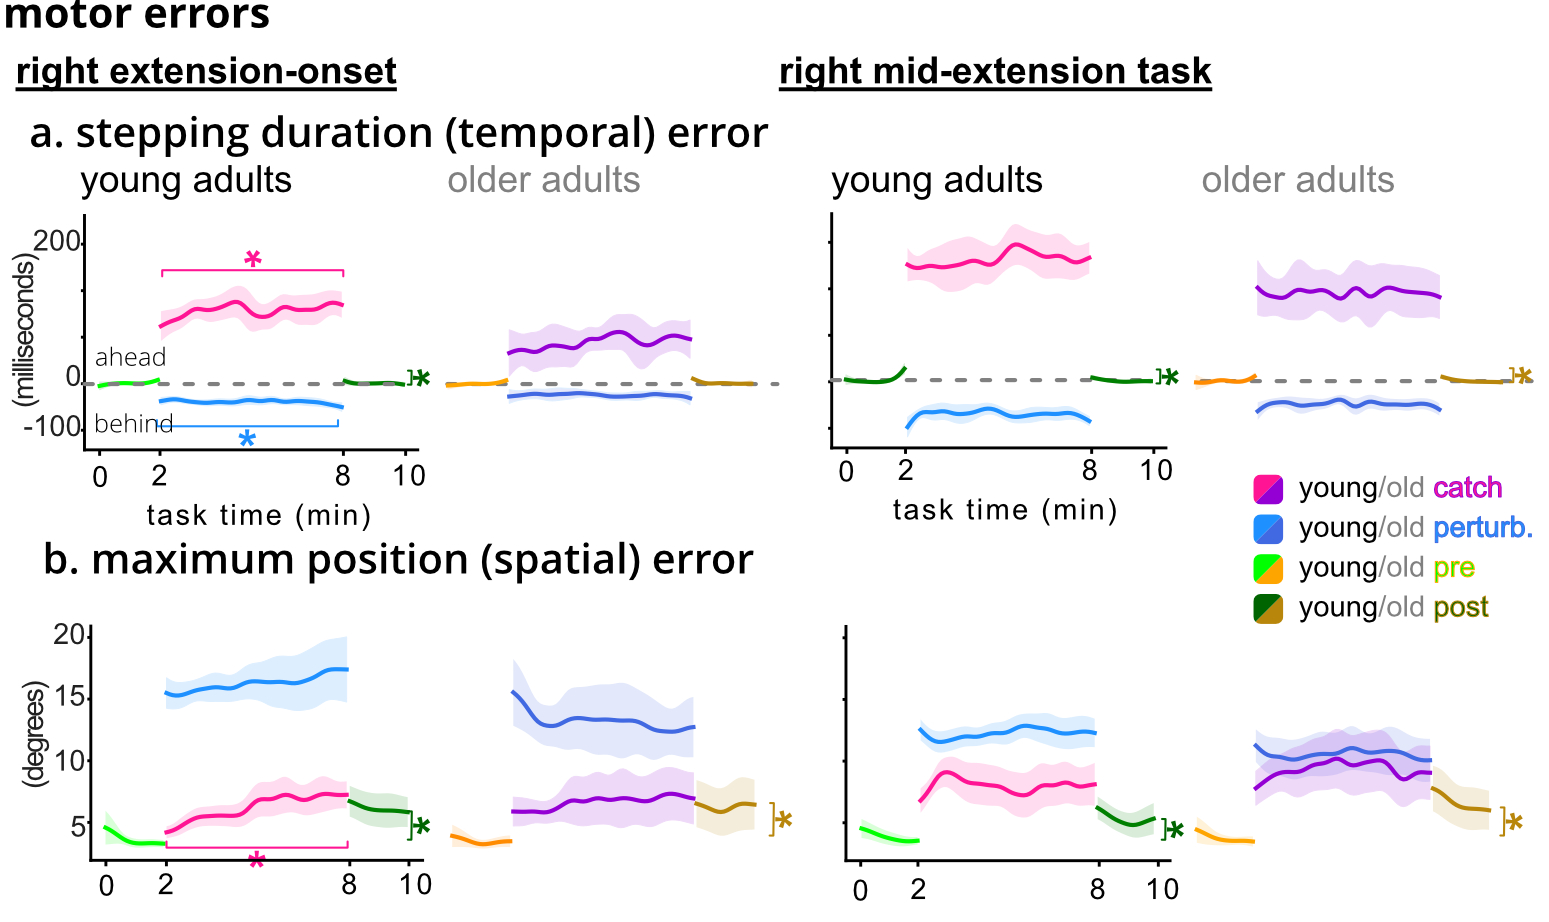
\includegraphics[scale=1]{../img/S1_error-metrics.jpg}
    \caption{Motor errors for the right-side tasks}
    \label{fig:S1}
\end{figure}
\newpage
\begin{figure}[H]
    \centering
    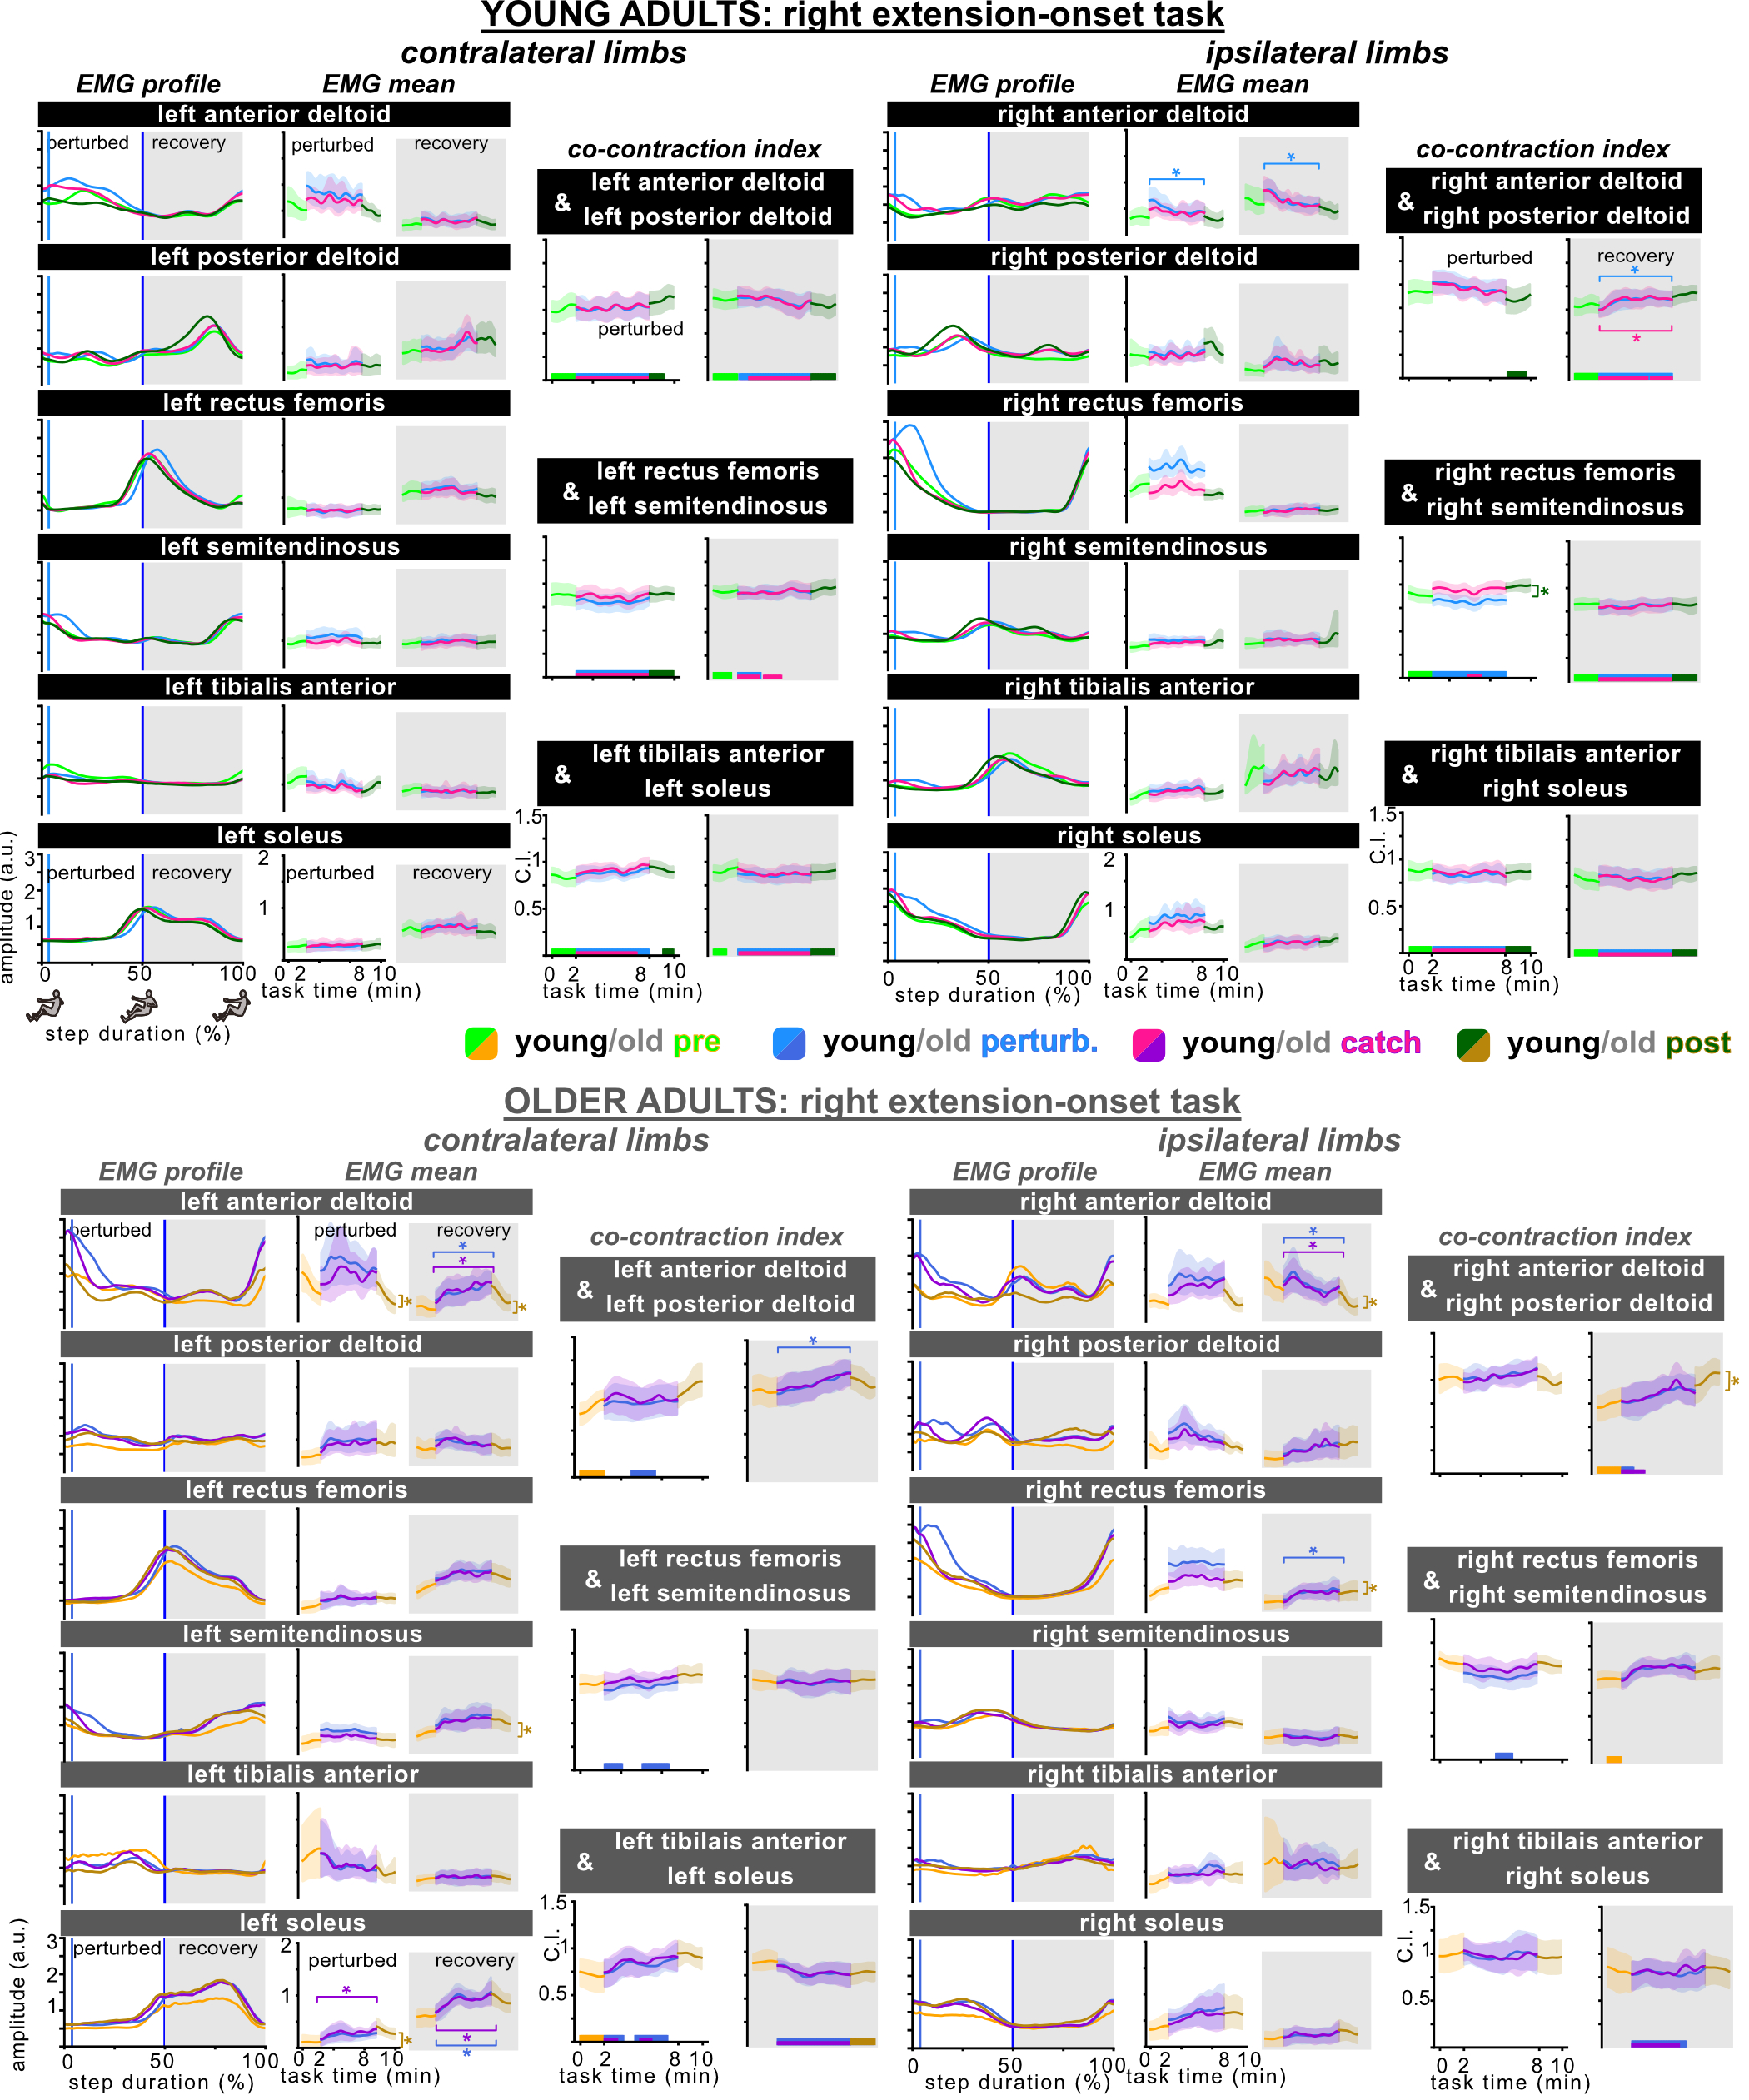
\includegraphics[scale=.9]{../img/S2_REI-EMG-CoCont.jpg}
    \caption{EMG profiles (i.e., linear envelopes), time course of the EMG means for each block, and the time course co-contraction indices for the \textbf{right extension-onset} task.}
    \label{fig:S2}
\end{figure}
\newpage
\begin{figure}[H]
    \centering
    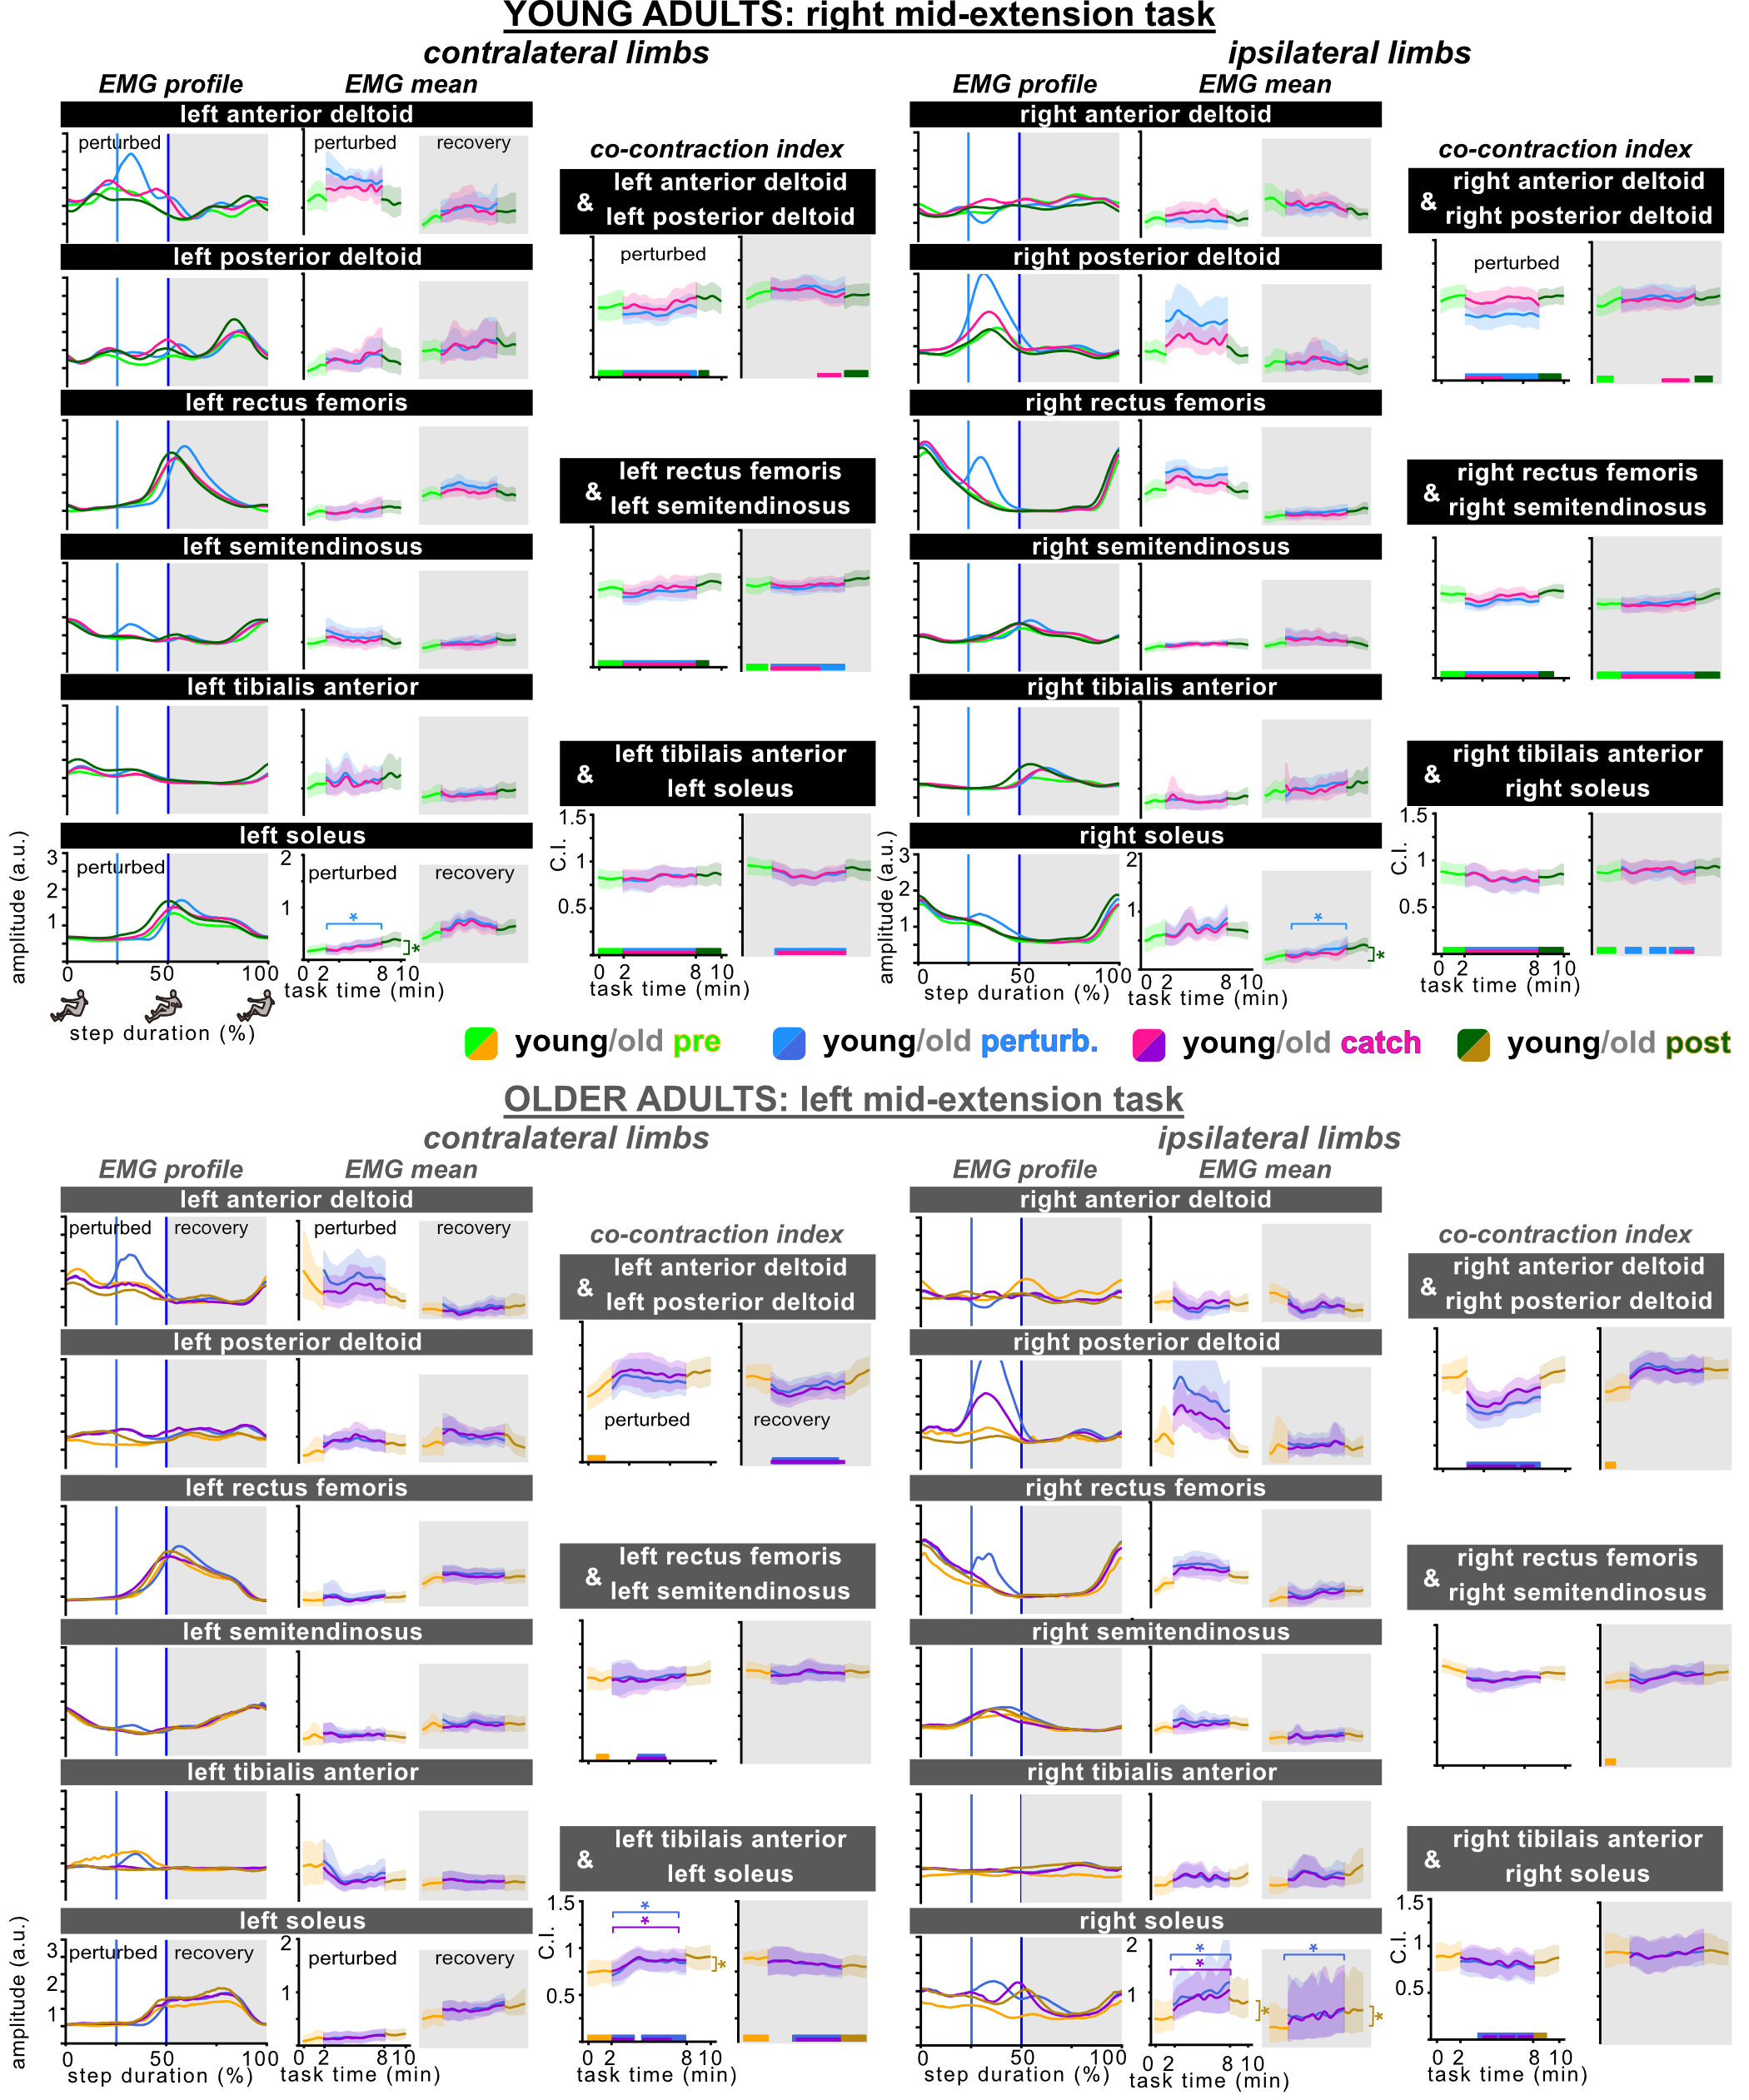
\includegraphics[scale=.9]{../img/S3_RME-EMG-CoCont.jpg}
    \caption{EMG profiles (i.e., linear envelopes), time course of the EMG means for each block, and the time course co-contraction indices for the \textbf{right mid-extension} task.}
    \label{fig:S3}
\end{figure}
\newpage
\begin{figure}[H]
    \centering
    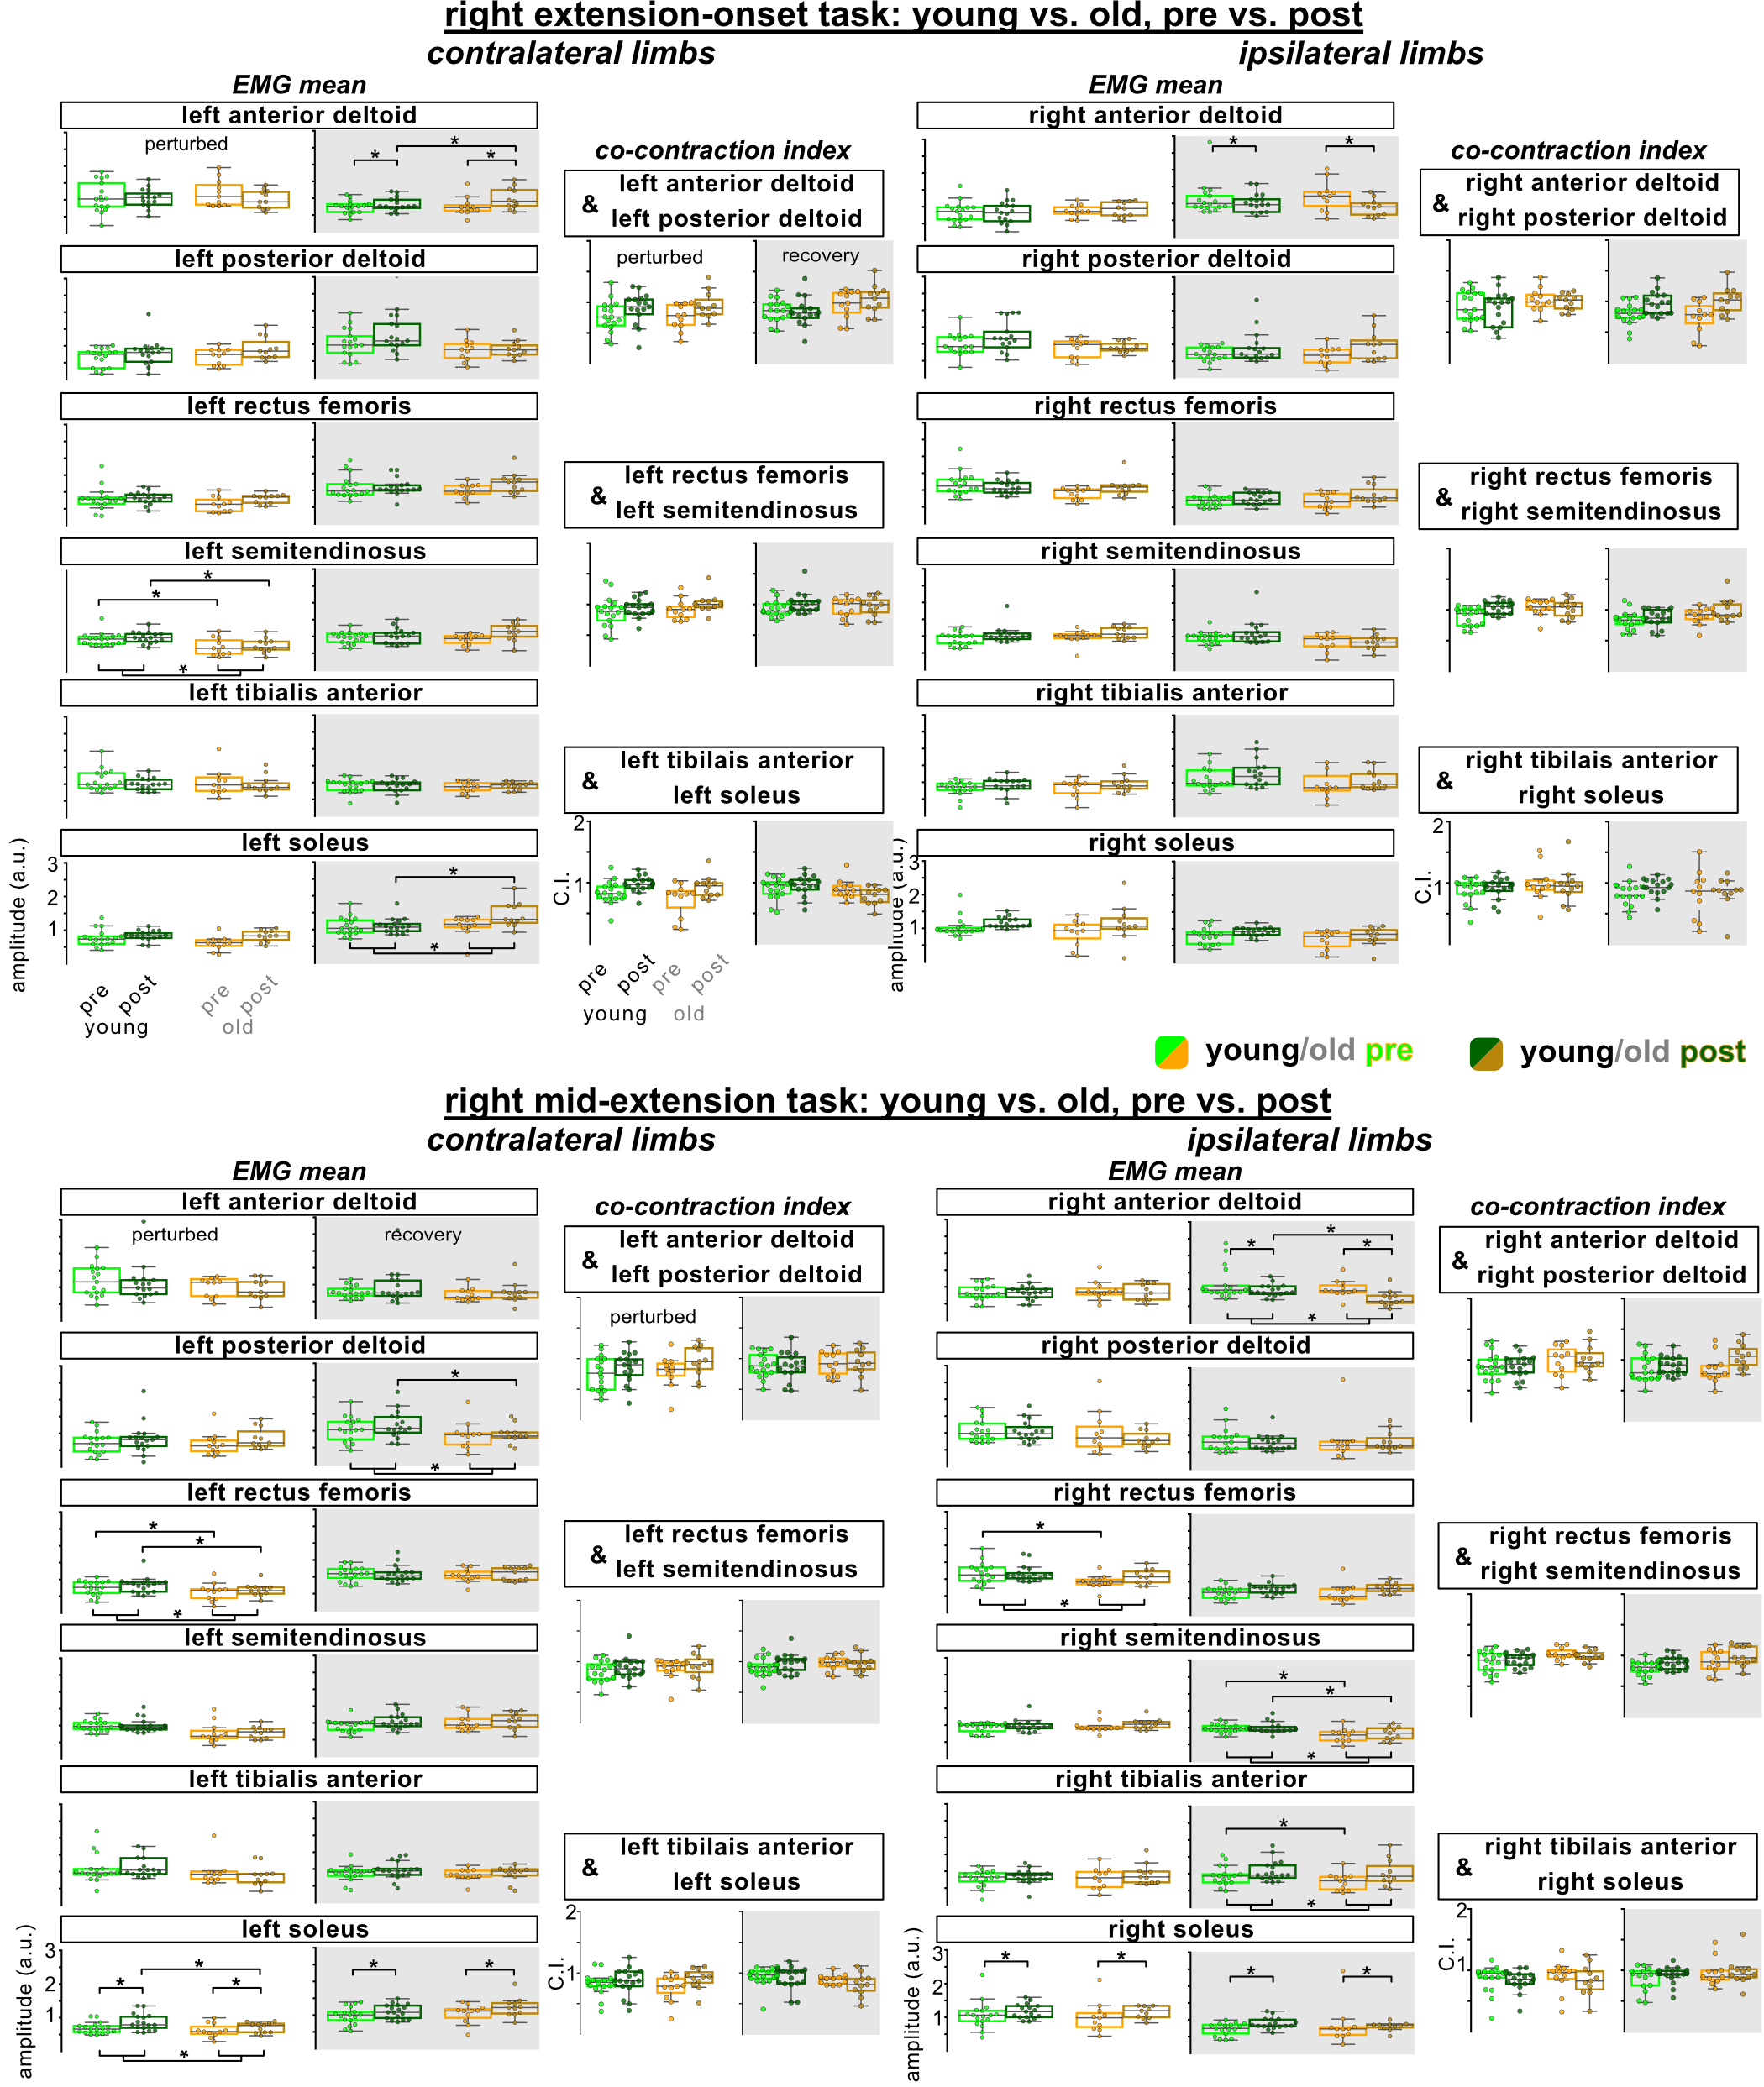
\includegraphics[scale=.9]{../img/S4_rightside_pre-post-comparison.jpg}
    \caption{Comparison of mean EMG and co-contraction between pre and post for the \textbf{right-side} tasks.}
    \label{fig:S4}
\end{figure}

% \printbibliography
\end{document}